% ResearchPhO solutions: How does disorder enter a model, a Hall current and a pump?
% Answers + marking scheme per problem; research context in Appendices A-E. Compile twice with pdflatex.
\documentclass[11pt,a4paper]{article}
\usepackage[T1]{fontenc}
\usepackage[utf8]{inputenc}
\usepackage{fix-cm}
\usepackage[scaled=0.96]{helvet}
\renewcommand{\familydefault}{\sfdefault}
\usepackage{amsmath,amssymb,mathtools}
\usepackage{newtxmath}
\usepackage{bm,dsfont}
\usepackage[margin=20mm,top=35mm,bottom=20mm,headheight=57pt,headsep=10mm]{geometry}
\usepackage{microtype,booktabs,array,tabularx,enumitem,needspace,longtable}
\usepackage[most]{tcolorbox}
\usepackage{fancyhdr,xcolor}
\usepackage{tikz}
\usetikzlibrary{arrows.meta,calc,positioning,shapes.geometric}
\usepackage{pgfplots}
\pgfplotsset{compat=1.18}
\usepackage[hidelinks,pdfencoding=auto,psdextra]{hyperref}
\hypersetup{pdftitle={ResearchPhO: How does disorder enter a model, a Hall current and a pump? - Solutions},pdfsubject={ResearchPhO: research-based exam in IPhO/APhO format}}
\definecolor{ink}{HTML}{172A3A}
\definecolor{rulegray}{HTML}{5E6670}
\definecolor{sourcegreen}{HTML}{1B6B4B}
\definecolor{sourcewash}{HTML}{F4FAF6}
\definecolor{openred}{HTML}{A42B32}
\definecolor{openwash}{HTML}{FFF6F6}
\definecolor{colA}{HTML}{D9822B}
\definecolor{colB}{HTML}{3C78B4}
\definecolor{amber}{HTML}{B7791F}
\setlength{\parindent}{0pt}
\setlength{\parskip}{5.4pt}
\setlength{\emergencystretch}{2em}
\setlength{\abovedisplayskip}{6pt}
\setlength{\belowdisplayskip}{6pt}
\raggedbottom
\newcounter{problemno}
\newcounter{figc}
\renewcommand{\thefigc}{\ifnum\value{problemno}=0 A\else\arabic{problemno}\fi.\arabic{figc}}
\newcommand{\pagecode}{S0}
\renewcommand{\thepage}{\pagecode-\arabic{page}}
\pagestyle{fancy}
\fancyhf{}
\fancyhead[L]{\begin{minipage}[b]{0.73\textwidth}\textbf{\large Solutions and Marking Scheme}\\[-1pt]{\small ResearchPhO \enspace|\enspace Solutions}\\[-1pt]{\footnotesize English}\end{minipage}}
\fancyhead[R]{\fontsize{29}{31}\selectfont\bfseries \thepage}
\renewcommand{\headrulewidth}{0.9pt}
\fancyfoot[L]{\footnotesize ResearchPhO --- a research-based exam in IPhO/APhO format}
\newcommand{\ket}[1]{\lvert #1\rangle}
\newcommand{\bra}[1]{\langle #1\rvert}
\newcommand{\Tr}{\operatorname{Tr}}
\newcommand{\dd}{\mathrm d}
\newcommand{\id}{\mathds 1}
\newcommand{\hc}{\mathrm{h.c.}}
\newcommand{\avg}[1]{\overline{#1}}
\newcommand{\Var}{\operatorname{Var}}
\newcommand{\Cov}{\operatorname{Cov}}
\newcommand{\eF}{\varepsilon_{\rm F}}
\newcommand{\problemsol}[3]{\clearpage\setcounter{problemno}{#1}\renewcommand{\pagecode}{S#1}\setcounter{page}{1}\setcounter{figc}{0}{\LARGE\bfseries\color{ink}Problem #1: #2}\hfill{\large\bfseries(#3 points)}\par\medskip}
\newcommand{\appendixstart}{\clearpage\renewcommand{\pagecode}{SA}\setcounter{page}{1}\setcounter{problemno}{0}\setcounter{figc}{0}}
\newcommand{\parttitle}[3]{\par\Needspace{8\baselineskip}\vspace{6pt}{\large\bfseries\color{ink}Part #1. #2\hfill\normalsize(#3 points)}\par\vspace{2pt}}
\newcommand{\pagetitle}[1]{{\large\bfseries\color{ink}#1}\par\vspace{4pt}}
\newcommand{\smallheading}[1]{\par\Needspace{6\baselineskip}\medskip\textbf{#1}\par}
\newcommand{\soltitle}[3]{\par\Needspace{4\baselineskip}{\bfseries\color{ink}#1\quad #3}\hfill{\small\bfseries #2 pt}\par}
\newcommand{\marking}[1]{\par{\footnotesize\textit{Marking: #1}}\par}
\newenvironment{figpanel}[1]{\refstepcounter{figc}\gdef\figtitle{#1}\par\medskip\noindent\begin{minipage}{\linewidth}\centering}{\end{minipage}\par\medskip}
\newcommand{\figtext}[1]{\par\smallskip{\raggedright\small\textbf{Figure \thefigc.} \figtitle. #1\par}}
\newtcolorbox{greenbox}[1]{enhanced,breakable,colback=sourcewash,colframe=sourcegreen,boxrule=0.9pt,arc=0pt,left=8pt,right=8pt,top=6pt,bottom=6pt,title={\strut AVAILABLE --- #1},colbacktitle=sourcewash,coltitle=sourcegreen,fonttitle=\bfseries\small,titlerule=0pt,fontupper=\small}
\newtcolorbox{redbox}[1]{enhanced,breakable,colback=openwash,colframe=openred,boxrule=0.9pt,arc=0pt,left=8pt,right=8pt,top=6pt,bottom=6pt,title={\strut NOT ESTABLISHED --- #1},colbacktitle=openwash,coltitle=openred,fonttitle=\bfseries\small,titlerule=0pt,fontupper=\small}
\newcolumntype{Y}{>{\raggedright\arraybackslash}X}
\pgfplotsset{mbaxis/.style={width=7.6cm,height=5.4cm,tick label style={font=\scriptsize},label style={font=\small},axis line style={rulegray},tick style={rulegray},legend style={font=\scriptsize,draw=none,fill=none}}}
\tikzset{>={Stealth[length=2.2mm]},
  obj/.style={draw=ink,rounded corners=2pt,align=center,font=\scriptsize,inner sep=3pt,text width=40mm,fill=white},
  okarrow/.style={->,draw=ink,line width=0.8pt},
  calcarrow/.style={->,draw=amber,dashed,line width=0.9pt},
  openarrow/.style={->,draw=openred,dashed,line width=0.9pt}}
\begin{document}

{\LARGE\bfseries\color{ink}How does disorder enter a model, a Hall current and a pump?}\par
{\large ResearchPhO --- Solutions and marking scheme \hfill \textbf{30 points}}

\smallheading{How to use this booklet}
Each answer is followed by its marking scheme; the numbers in a marking line add up to the points of the question. (M) marks a modelling step: setting up the model, choosing the physics, interpreting a result, judging its scope. (C) marks a computation step: algebra, solving, evaluating. Most of each problem's marks go to (M). Give partial credit for a correct approximate route. Appendices A--D contain the research context; Appendix E, the toolbox, gives the smallest worked example of each tool from ``Useful information''. Every number in this booklet is recomputed by the answer script of the working folder.

\smallheading{Mark allocation}
{\small\begin{tabularx}{\textwidth}{@{}p{18mm}Y r@{}}\toprule
Problem&Questions&Points\\\midrule
1&A.1 (1.2), A.2 (1.2), B.1 (1.2), B.2 (1.0), C.1 (1.3), C.2 (1.1), C.3 (0.8), D.1 (1.0), D.2 (0.8), D.3 (0.4)&10.0\\
2&A.1 (0.9), A.2 (0.5), A.3 (0.8), B.1 (0.9), B.2 (1.2), B.3 (0.7), C.1 (0.9), C.2 (0.8), C.3 (1.1), D.1 (0.8), D.2 (0.9), D.3 (0.5)&10.0\\
3&A.1 (0.8), A.2 (0.8), B.1 (1.0), B.2 (1.0), C.1 (1.2), C.2 (0.8), C.3 (0.6), D.1 (0.6), D.2 (1.2), D.3 (1.0), D.4 (1.0)&10.0\\\midrule
&&\textbf{30.0}\\\bottomrule
\end{tabularx}}

%%%%%%%%%%%%%%%%%%%%%%%%%%%%%%%%%%%%%%%%%%%%%%%%%%%%%%%%%%%%%%%%%%%%%%%%%%%%%%%%%%%%%%%%%%%%%%%%
\problemsol{1}{From a dirty crystal to a random Hamiltonian}{10.0}

\parttitle{A}{From an impurity to lattice parameters}{2.4}
\soltitle{A.1}{1.2}{One impurity changes several matrix elements at once}
\textbf{(a)} The delta function gives $\delta h_{ij}=u_0\,\varphi_i(x_0)\varphi_j(x_0)$. With $\varphi_j(ja)=(\pi b^2)^{-1/4}$ and $\varphi_{j+1}(ja)=(\pi b^2)^{-1/4}e^{-a^2/(2b^2)}$:
\[
x_0=ja:\quad \delta h_{jj}=\frac{u_0}{\sqrt\pi\,b},\qquad
\delta h_{j,j+1}=\frac{u_0}{\sqrt\pi\,b}\,e^{-a^2/(2b^2)},\qquad
\delta h_{j+1,j+1}=\frac{u_0}{\sqrt\pi\,b}\,e^{-a^2/b^2}.
\]
Midway, $\varphi_j(x_0)=\varphi_{j+1}(x_0)=(\pi b^2)^{-1/4}e^{-a^2/(8b^2)}$, so
\[
x_0=(j+\tfrac12)a:\quad \delta h_{jj}=\delta h_{j+1,j+1}=\delta h_{j,j+1}=\frac{u_0}{\sqrt\pi\,b}\,e^{-a^2/(4b^2)}.
\]
\textbf{(b)} On the atom, $|\delta h_{j,j+1}/\delta h_{jj}|=e^{-a^2/(2b^2)}=e^{-8}=\boxed{3\times10^{-4}}$ (and the neighbour's on-site term is $e^{-16}\approx10^{-7}$ of it). With orthogonalized orbitals this small ratio becomes of the order of the overlap $e^{-a^2/(4b^2)}\approx0.02$: still small. Midway, the ratio is $\boxed{1}$. An impurity on an atom is well described by one random on-site energy: the Anderson model is adequate when impurities sit on (or near) atoms and the orbitals are compact, $b\ll a$. An impurity between atoms changes two on-site energies and the hopping between them by the same amount; a model with random on-site energies only misses half of its effect.

\textbf{(c)} $\delta h_{ij}=u_0\,\phi_i\phi_j$ with the vector $\phi_i=\varphi_i(x_0)$: $\delta h=u_0\,\phi\phi^{T}$, a matrix of rank one. All its entries are fixed by the same two random numbers $(u_0,x_0)$. The on-site and bond terms of one impurity are therefore perfectly correlated (with the sign of $u_0$); drawing them as independent random numbers misrepresents the ensemble. The correct procedure samples the \emph{source} (impurity strength and position) and computes all matrix elements from it.
\marking{(a) The matrix elements: 0.35 (C). (b) The two ratios: 0.15 (C); adequacy of the on-site model for each kind: 0.3 (M). (c) Rank one: 0.1 (C); correlated channels, sample the source and not the matrix elements: 0.3 (M).}

\soltitle{A.2}{1.2}{Equal variances do not mean equal disorder}
\textbf{(a)} $\avg{\epsilon_j}=f_{\rm s}\epsilon_{\rm s}$; $\kappa_2=f_{\rm s}(1-f_{\rm s})\epsilon_{\rm s}^2$;
\[
\kappa_3=(1-f_{\rm s})(-f_{\rm s}\epsilon_{\rm s})^3+f_{\rm s}\big((1-f_{\rm s})\epsilon_{\rm s}\big)^3=f_{\rm s}(1-f_{\rm s})\big[(1-f_{\rm s})^2-f_{\rm s}^2\big]\epsilon_{\rm s}^3=\boxed{f_{\rm s}(1-f_{\rm s})(1-2f_{\rm s})\epsilon_{\rm s}^3}.
\]
The mean shifts all orbital energies by the same $f_{\rm s}\epsilon_{\rm s}$, so it shifts the band rigidly. It is absorbed into the chemical potential (or into the clean Hamiltonian); the disorder model keeps only $\epsilon_j-f_{\rm s}\epsilon_{\rm s}$, which has zero mean.

\textbf{(b)} $f_{\rm s}(1-f_{\rm s})\epsilon_{\rm s}^2=W^2/12$ gives $\epsilon_{\rm s}=W/\sqrt{12f_{\rm s}(1-f_{\rm s})}$, i.e.\ $\epsilon_{\rm s}/W=\boxed{0.962}$ at $f_{\rm s}=0.1$, and
\[
\frac{\kappa_3}{W^3}=\frac{1-2f_{\rm s}}{12^{3/2}\sqrt{f_{\rm s}(1-f_{\rm s})}}=\frac{0.8}{41.57\times0.3}=\boxed{0.064}.
\]
$\kappa_3=0$ at $f_{\rm s}=\boxed{1/2}$ (model 1 has $\kappa_3=0$ for every $W$).

\textbf{(c)} A third-order quantity contains averages of three random energies, for example $\avg{\epsilon_j\epsilon_l\epsilon_m}$, which is non-zero only for $j=l=m$ and equals $\kappa_3$: the electron visits the same atom three times (in a scattering amplitude, the interference of $V$ with $VG_0V$). Model 1 gives zero, model 2 with $f_{\rm s}=0.1$ gives $0.064W^3$, so effects that first appear at third order, such as an asymmetry of scattering, exist only in model 2, although both models give the same second-order results (rates, broadening). Replacing $\epsilon_{\rm s}$ by $-\epsilon_{\rm s}$ leaves $\kappa_2$ unchanged and reverses the sign of $\kappa_3$: second-order results stay, third-order results change sign.
\marking{(a) The three cumulants: 0.3 (C); the mean is absorbed into the chemical potential: 0.2 (M). (b) $\epsilon_{\rm s}/W$, $\kappa_3/W^3$ and $f_{\rm s}=1/2$: 0.25 (C). (c) Third-order quantities need $\kappa_3$: 0.3 (M); effect of $\epsilon_{\rm s}\to-\epsilon_{\rm s}$: 0.15 (M).}

\parttitle{B}{Displaced atoms}{2.2}
\soltitle{B.1}{1.2}{Position disorder gives correlated bonds}
\textbf{(a)} $d_j=a+u_{j+1}-u_j$, so $\delta J_j=J'(a)(u_{j+1}-u_j)$. Then $\Var(\delta J_j)=2J'^2\sigma_u^2$; bonds $j$ and $j+1$ share atom $j+1$, so $\Cov(\delta J_j,\delta J_{j+1})=-J'^2\sigma_u^2$ (correlation coefficient $-1/2$); $\Cov(\delta J_j,\delta J_{j+n})=0$ for $n\ge2$.

\textbf{(b)} $K_J(q)=2J'^2\sigma_u^2-J'^2\sigma_u^2(e^{iq}+e^{-iq})=\boxed{2J'^2\sigma_u^2(1-\cos q)=4J'^2\sigma_u^2\sin^2(q/2)}$, so $K_J(0)=0$. The sum telescopes: $\sum_{j=1}^{M}\delta J_j=J'(a)(u_{M+1}-u_1)$, with variance $2J'^2\sigma_u^2$ for every $M$. The total length of a stretch of bonds is the distance between its two end atoms; lengthening one bond shortens its neighbours. Long-wavelength variations of the bond lengths are absent.

\textbf{(c)} Independent bonds: $K_J(q)=2J'^2\sigma_u^2$ for every $q$ (white noise) and $\Var\sum_{j=1}^M\delta J_j=2MJ'^2\sigma_u^2$. The average hopping (the local bandwidth) of a stretch of $M$ bonds therefore fluctuates by $\propto M^{-1/2}$ in the independent model, but only by $\propto M^{-1}$ with position disorder. Equivalently, scattering with small momentum transfer $q$ and slow variations of the bandwidth are present in one model and absent in the other.
\marking{(a) Linearization through the shared atoms: 0.15 (M); the three covariances: 0.25 (C). (b) $K_J(q)$ and $K_J(0)=0$: 0.15 (C); telescoping sum and its physical reason: 0.3 (M). (c) The independent model: 0.1 (C); the two scalings of the average hopping: 0.25 (M).}

\soltitle{B.2}{1.0}{Hopping and interaction move together}
\textbf{(a)} $J\propto r^{-3}$ and $V_6\propto r^{-6}$ give
\[
\frac{\delta J_j}{J(a)}=-\frac{3(u_{j+1}-u_j)}{a},\qquad\frac{\delta V_{6,j}}{V_6(a)}=-\frac{6(u_{j+1}-u_j)}{a}.
\]
Both are multiples of the same variable with coefficients of the same sign: the correlation coefficient is $\boxed{+1}$. The rms values are $3\sqrt2\,\sigma_u/a=\boxed{0.127}$ and $6\sqrt2\,\sigma_u/a=\boxed{0.255}$.

\textbf{(b)} $\avg{J(d_j)}\approx J(a)+\tfrac12J''(a)\avg{(u_{j+1}-u_j)^2}$ with $J''/J=12/a^2$ and $V_6''/V_6=42/a^2$:
\[
\frac{\avg{J_j}}{J(a)}-1=\frac{12\sigma_u^2}{a^2}=\boxed{1.1\%},\qquad\frac{\avg{V_{6,j}}}{V_6(a)}-1=\frac{42\sigma_u^2}{a^2}=\boxed{3.8\%}.
\]
(A Monte Carlo average of the exact functions gives 1.09\% and 3.9\%.) Because $J(r)$ and $V_6(r)$ are convex, disorder increases their means: the clean values are not the averages.

\textbf{(c)} Any two of: the perfect correlation of $J_j$ and $V_{6,j}$ (a short bond has both a large hopping and a large interaction); the anticorrelation of neighbouring bonds and the absence of long-wavelength fluctuations (B.1); the shifted means of (b).
\marking{(a) The two relative changes: 0.2 (C); correlation $+1$: 0.15 (M); rms values: 0.1 (C). (b) Mean shifts: 0.2 (C); the convex dependence shifts the mean: 0.1 (M). (c) Two missed features: 0.25 (M).}

\parttitle{C}{From correlations to rates}{3.2}
\soltitle{C.1}{1.3}{Golden-rule rate, broadening, mean free path --- and their limit}
\textbf{(a)} $V_{k'k}=\frac1L\sum_j\epsilon_je^{i(k-k')j}$, so
\[
\avg{|V_{k'k}|^2}=\frac1{L^2}\sum_{j,l}\avg{\epsilon_j\epsilon_l}e^{i(k-k')(j-l)}=\frac1{L^2}\sum_j\avg{\epsilon_j^2}=\frac{W^2}{12L}.
\]
\textbf{(b)} $\frac1\tau=\frac{2\pi}\hbar\sum_{k'}\frac{W^2}{12L}\delta(E-E_{k'})=\frac{2\pi}{\hbar}\frac{W^2}{12}\nu(E)$. At $E=J$, $\nu=1/(\pi\sqrt3J)$:
\[
\frac1\tau=\frac{W^2}{6\sqrt3\,\hbar J},\qquad
\Gamma=\frac\hbar{2\tau}=\frac{W^2}{12\sqrt3\,J}=\boxed{0.048\,J},\qquad
\ell=|v_k|\tau=\sqrt3\frac{Ja}{\hbar}\cdot\frac{6\sqrt3\hbar J}{W^2}=\frac{18J^2a}{W^2}=\boxed{18\,a}
\]
for $W=J$. (An exact time evolution of a plane wave on a 3000-site ring at $W=0.5J$ gives a decay rate within 3\% of this formula.)

\textbf{(c)} $\xi=24\cdot3J^2a/W^2=72J^2a/W^2$, so $\xi/\ell=\boxed{4}$: the waves are localized after a few mean free paths. For $L_{\rm w}=1000a\gg\xi=72a$: $e^{-2L_{\rm w}/\xi}=e^{-27.8}\approx\boxed{9\times10^{-13}}$, whereas $\ell/L_{\rm w}=\boxed{0.018}$ (both in units of $e^2/h$). The $\tau$-based estimate is wrong by ten orders of magnitude: $\tau$ contains no interference. The decisive comparison is $L_{\rm w}$ versus $\xi$ ($\tau$ alone is meaningful only for $L_{\rm w}\ll\xi$). At finite temperature, if $\ell\ll L_\varphi\ll\xi$, interference is cut off before it localizes the electron, and a $\tau$-based description holds on scales larger than $L_\varphi$.
\marking{(a) Average over independent energies: 0.2 (C). (b) Rate from the density of final states: 0.2 (M); $1/\tau$, $\Gamma$ and $\ell$ with numbers: 0.3 (C). (c) $\xi/\ell=4$ and the two conductances: 0.1 (C); $L_{\rm w}\gg\xi$, localized, $\tau$ alone meaningless, the decisive comparison: 0.3 (M); condition $\ell\ll L_\varphi\ll\xi$: 0.2 (M).}

\soltitle{C.2}{1.1}{Same broadening, different mobility}
\textbf{(a)} For $\lambda\to0$, $K_U$ is constant; $\int_{-\pi}^{\pi}\dd\theta=\int_{-\pi}^{\pi}(1-\cos\theta)\dd\theta=2\pi$, so $\tau_{\rm tr}/\tau_q=\boxed1$.

\textbf{(b)} For $k_{\rm F}\lambda\gg1$ only small angles contribute: $Q^2\approx k_{\rm F}^2\theta^2$, $K_U\propto e^{-\alpha\theta^2/2}$ with $\alpha=(k_{\rm F}\lambda)^2$, $1-\cos\theta\approx\theta^2/2$, and the limits can be extended to $\pm\infty$:
\[
\frac{\tau_{\rm tr}}{\tau_q}=\frac{\int e^{-\alpha\theta^2/2}\dd\theta}{\int e^{-\alpha\theta^2/2}\,\frac{\theta^2}2\,\dd\theta}=\frac{\sqrt{2\pi/\alpha}}{\frac12\sqrt{2\pi/\alpha}/\alpha}=2\alpha=2(k_{\rm F}\lambda)^2 .
\]
\textbf{(c)} At equal $\tau_q$, the mobility ratio is the ratio of $\tau_{\rm tr}$: $2\times3^2=\boxed{18}$ (the exact angular integral gives 17.4), in favour of the smooth disorder. A broadening $\Gamma$ added to a clean formula captures the lifetime of a momentum state (the width of a spectral line). It misses the angular distribution of the scattering, which decides how fast the current direction is lost (the transport time; in diagrammatic language, vertex corrections), and every effect beyond second order in the random potential.
\marking{(a) 0.15 (C). (b) Small-angle reduction: 0.2 (M); Gaussian integrals: 0.2 (C). (c) Ratio 18: 0.15 (C); what $\Gamma$ captures and what it misses: 0.4 (M).}

\soltitle{C.3}{0.8}{Static disorder alone does not make a decay}
\textbf{(a)} With $\Delta=\epsilon_1-\epsilon_2$,
\[
P_2(t)=\frac{4J^2}{\Delta^2+4J^2}\sin^2\!\Big(\frac{\sqrt{\Delta^2+4J^2}}{2\hbar}t\Big).
\]
It is bounded and periodic: the detuning reduces and speeds up the oscillation, but nothing leaves irreversibly. Static disorder is a unitary, time-independent part of $H$.

\textbf{(b)} (i) A decay at rate $1/\tau$ is seen only for $\tau\ll t\ll t_{\rm H}$; this needs $\tau\ll t_{\rm H}$, equivalently many levels within the width $\Gamma$. For later times the discrete spectrum gives recurrences. (ii) $\Gamma\ll4J$: the width must be small compared with the band width, over which $\nu(E)$ and the matrix elements change (weak disorder, $\ell\gg a$), so that second order is enough. At $E=J$, $L=1000$:
\[
t_{\rm H}=2\pi\hbar L\nu(J)=\frac{2000}{\sqrt3}\frac{\hbar}{J}=\boxed{1155\,\hbar/J}\gg\tau=6\sqrt3\,\hbar/J=10.4\,\hbar/J .
\]
\marking{(a) $P_2(t)$: 0.2 (C); no irreversible decay: 0.15 (M). (b) The two conditions: 0.3 (M); $t_{\rm H}$ and comparison: 0.15 (C).}

\parttitle{D}{Which random term first?}{2.2}
\soltitle{D.1}{1.0}{Size is not importance: spectrum and observation time}
\textbf{(a)} $S(\omega_0)\propto\tau_{\rm c}/(1+\omega_0^2\tau_{\rm c}^2)$ is maximal at $\tau_{\rm c}=1/\omega_0=\hbar/(10\text{ meV})=66$ fs, where $S=\sigma_\eta^2/\omega_0$:
\[
r_{10}^{\max}=\frac{|A_{10}|^2\sigma_\eta^2}{\hbar^2\omega_0}=\frac{(0.1\text{ meV})^2}{\hbar\cdot10\text{ meV}}=\frac{10^{-3}\text{ meV}}{\hbar}=\boxed{1.5\times10^{9}\ \text{s}^{-1}}.
\]
\textbf{(b)} $r_{10}=r^{\max}_{10}\,2\omega_0\tau_{\rm c}/(1+\omega_0^2\tau_{\rm c}^2)$ with $\omega_0=1.52\times10^{13}$ s$^{-1}$: $\tau_{\rm c}=1$ ns gives $\boxed{2.0\times10^5\ \text{s}^{-1}}$; $\tau_{\rm c}=1$ fs gives $\boxed{4.6\times10^7\ \text{s}^{-1}}$.

\textbf{(c)} $t_{\rm obs}=1$ ps: $1.5\times10^{-3}$, $2\times10^{-7}$, $4.6\times10^{-5}$ --- all negligible. $t_{\rm obs}=10\ \mu$s: $1.5\times10^{4}$, $2.0$, $4.6\times10^{2}$ --- all three matter. The same noise is irrelevant for an ultrafast measurement and decisive for a slow pump: the ranking depends on the observation time, not only on $\sigma_\eta$. For $\tau_{\rm c}=1$ ns and $t_{\rm obs}=1$ ps the noise is frozen during the measurement: it acts as a static random shift (part (d)), not as a rate.

\textbf{(d)} For $\tau_{\rm c}\to\infty$, $S(\omega_0)\approx2\sigma_\eta^2/(\omega_0^2\tau_{\rm c})\to0$: all the noise power sits at $\omega=0$ and causes no transitions between non-degenerate levels. Static disorder belongs in $H_{\mathcal C}$: solve (diagonalize, or expand) the Hamiltonian including it, compute the observable in each configuration, then average.

\textbf{(e)} The eigenstates have a definite electron number; $\ket0,\ket1$ belong to the same $N_0$, so $\langle1|\hat N|0\rangle=N_0\langle1|0\rangle=0$ and $r_{10}=\boxed0$ for any $\sigma_\eta$: the noise only adds a global phase. (If the sample exchanges electrons with leads, the same noise shifts its potential relative to them and does matter.)
\marking{(a) Optimal $\tau_{\rm c}$ and maximal rate: 0.2 (C). (b) The two rates: 0.15 (C). (c) The products: 0.1 (C); the importance depends on $t_{\rm obs}$, and frozen noise for $\tau_{\rm c}\gg t_{\rm obs}$: 0.2 (M). (d) No transitions; static disorder goes into $H_{\mathcal C}$: 0.2 (M). (e) Zero, and why: 0.15 (M).}

\soltitle{D.2}{0.8}{A mean shift survives averaging; the spread does not}
\textbf{(a)} $\chi''(\mu_0)=-2\chi_0/\Lambda^2$, so $\avg\chi/\chi_0-1\approx-\sigma_\mu^2/\Lambda^2=\boxed{-9\%}$ (the exact Gaussian average gives $-7.3\%$). At $\mu_0+\Lambda$: $\chi=\chi_0/2$ and $\chi'=-\chi_0/(2\Lambda)$, so the rms local variation is $\chi_0\sigma_\mu/(2\Lambda)$, i.e.\ $\sigma_\mu/\Lambda=\boxed{30\%}$ of $\chi(\mu_0+\Lambda)$.

\textbf{(b)} The mean shift survives: it is a bias of every puddle in the same direction. The variation of the spatial average over $N_{\rm p}$ independent puddles decreases as $N_{\rm p}^{-1/2}$ (self-averaging).

\textbf{(c)} Any two of: $\sigma_\mu\gtrsim\Lambda$ (the Taylor expansion fails; average the full function); a non-local response (puddles smaller than the mean free path or coherence length); non-uniform current paths and local fields (then solve $\nabla\cdot\bm j=0$ with the local coefficients, as in an effective-medium or resistor-network model); puddles comparable to the sample size (no self-averaging).
\marking{(a) Mean shift: 0.15 (C); relative spread at the flank: 0.15 (C). (b) Which survives, and $N_{\rm p}^{-1/2}$: 0.25 (M). (c) Two failure conditions: 0.25 (M).}

\soltitle{D.3}{0.4}{Three tests}
\begin{enumerate}[leftmargin=6mm,itemsep=1pt,topsep=1pt]
\item \emph{Coupling and symmetry:} compare the matrix element of the random term between the states that decide the observable with their energy separation, $|\langle n|\delta H|m\rangle|/|E_n-E_m|$, and check whether it breaks a symmetry the observable needs (A.1, D.1(e)).
\item \emph{Time scale:} compare its spectral weight at the relevant transition frequencies, times the observation time, with one ($r\,t_{\rm obs}$); a static term (all weight at $\omega=0$) goes into $H_{\mathcal C}$ (D.1).
\item \emph{Effect on the observable:} compare its mean shift and its sample-to-sample spread with the required accuracy, and check whether one rate or broadening is enough, or the angular structure, higher cumulants and interference are needed (A.2, C.1, C.2, D.2).
\end{enumerate}
\marking{Coupling test with its comparison: 0.15 (M). Time-scale test: 0.15 (M). Effect on the observable: 0.1 (M).}

%%%%%%%%%%%%%%%%%%%%%%%%%%%%%%%%%%%%%%%%%%%%%%%%%%%%%%%%%%%%%%%%%%%%%%%%%%%%%%%%%%%%%%%%%%%%%%%%
\problemsol{2}{Impurities and the second-order Hall current}{10.0}

\parttitle{A}{Three sources of a Hall current}{2.2}
\soltitle{A.1}{0.9}{Intrinsic Hall conductivity of one cone}
\textbf{(a)} $\bm d=(vk_x,vk_y,m)$, $\partial_{k_x}\bm d\times\partial_{k_y}\bm d=(0,0,v^2)$, $\bm d\cdot(\dots)=mv^2$:
\[
\Omega_\pm(\bm k)=\mp\frac{mv^2}{2\varepsilon_{\bm k}^3}=\mp\frac{mv^2}{2(v^2k^2+m^2)^{3/2}}.
\]
\textbf{(b)} The anomalous velocity is $-\dot{\bm k}\times\Omega\hat{\bm z}=(e/\hbar)\bm E\times\Omega\hat{\bm z}$; for $\bm E=E_x\hat{\bm x}$, $\hat{\bm x}\times\hat{\bm z}=-\hat{\bm y}$, so $\dot y_{\rm an}=-(e/\hbar)E_x\Omega$ and $j_y=-e\sum_n\int f_{0,n}\dot y_{\rm an}=(e^2/\hbar)E_x\sum_n\int f_{0,n}\Omega_n$. With $\int\frac{\dd^2k}{(2\pi)^2}=\frac1{2\pi}\int k\,\dd k$ and $\int_0^{k_1}\frac{v^2k\,\dd k}{\varepsilon_{\bm k}^3}=\frac1m-\frac1{\varepsilon_{k_1}}$:
\[
\text{lower band (all $k$)}:\ \frac{m}{4\pi}\cdot\frac1m=\frac1{4\pi};\qquad
\text{upper band ($k<k_{\rm F}$)}:\ -\frac m{4\pi}\Big(\frac1m-\frac1{\eF}\Big).
\]
The sum is $m/(4\pi\eF)$, so
\[
\sigma_{yx}=\frac{e^2}\hbar\frac m{4\pi\eF}=\boxed{\frac{e^2}{h}\,\frac{m}{2\eF}}.
\]
The filled lower band gives half a conductance quantum; the occupied part of the upper band reduces it.
\marking{(a) 0.15 (C). (b) The anomalous current summed over the occupied states of both bands: 0.3 (M); the two band integrals: 0.25 (C); result in $e^2/h$: 0.1 (C); reading of the two band contributions: 0.1 (M).}

\soltitle{A.2}{0.5}{Time reversal cancels the linear Hall current}
With $\bm k\to-\bm k$,
$\int\tilde f_0\tilde\Omega\,\dd^2k=-\int f_0(-\bm k)\Omega(-\bm k)\,\dd^2k=-\int f_0\Omega\,\dd^2k$: the partner gives $-\sigma_{yx}$ and the total vanishes. The Berry curvature is odd under time reversal; any Hall conductivity linear in $\bm E$ is odd under time reversal and therefore vanishes in a time-reversal-symmetric crystal, whatever its microscopic source.
\marking{Change of variables: 0.2 (C). The general statement: 0.3 (M).}

\soltitle{A.3}{0.8}{Three of four linear mechanisms scale alike}
Because $1/\tau\propto n_i$, each factor $n_i$ counts as $\tau^{-1}$; the linear distribution change is $\delta f\propto\tau E$.
\begin{center}\small\begin{tabular}{lll}\toprule
intrinsic&$f_0\times$ anomalous velocity&$\tau^0$\\
side jump&$\delta f\times v^{\rm sj}\propto\tau\cdot\tau^{-1}$&$\tau^0$\\
extrinsic skew&$g\propto\tau\,w_A^{(3)}\delta f\propto\tau\cdot n_i\cdot\tau$&$\tau^1$\\
intrinsic skew&$g\propto\tau\cdot n_i^2\cdot\tau$&$\tau^0$\\\bottomrule
\end{tabular}\end{center}
Intrinsic, side-jump and intrinsic-skew contributions all scale as $\tau^0$: changing $n_i$ cannot separate them. Only extrinsic skew scattering ($\propto\tau\propto\sigma_{xx}$) is separable; this is the origin of fits of the form $\sigma_{\rm AH}=a\,\sigma_{xx}+b$.
\marking{Counting impurity factors as powers of $\tau$: 0.2 (M). The four powers: 0.3 (C). Which cannot be separated: 0.3 (M).}

\parttitle{B}{A dipole of curvature}{2.8}
\soltitle{B.1}{0.9}{The curvature-dipole current}
The Hall part at second order is $f_1$ times the anomalous velocity:
\[
j_y=-e\int f_1\Big(-\frac e\hbar E_x\Omega\Big)=\frac{e^3\tau}{\hbar^2}E_x^2\int\Omega\,\partial_{k_x}f_0=-\frac{e^3\tau}{\hbar^2}D_xE_x^2,
\]
using integration by parts (summed over bands). For the partner, $\partial_{k_x}[\Omega(-\bm k)]=-(\partial_{k_x}\Omega)(-\bm k)$, so $\tilde D_x=\int f_0(-\bm k)(\partial_{k_x}\Omega)(-\bm k)\,\dd^2k/(2\pi)^2=D_x$: the two cones add. Time reversal makes $\Omega$ odd and $f_0$ even in $\bm k$, so $\int f_0\Omega$ cancels between partners; the field-shifted distribution $f_1\propto\partial_{k_x}f_0$ is odd, and its product with the odd $\Omega$ is even and survives.
\marking{Second-order current: 0.3 (C). Partner adds: 0.2 (C). Only $f_1$ times the anomalous velocity is the Hall part: 0.1 (M). Why time reversal allows it: 0.3 (M).}

\soltitle{B.2}{1.2}{Dipole of the tilted cone}
$\Omega$ does not depend on $v_t$ (the tilt multiplies the identity). For the upper band
\[
f_0=\Theta(\eF-\varepsilon_{\bm k}-v_tk_x)\approx\Theta(\eF-\varepsilon_{\bm k})-v_tk_x\,\delta(\varepsilon_{\bm k}-\eF).
\]
The zeroth-order term gives zero: $\Theta(\eF-\varepsilon_{\bm k})$ is even and $\partial_{k_x}\Omega$ odd in $k_x$. With $\partial_{k_x}\Omega=\Omega'(k)k_x/k$ and $\Omega'(k)=3mv^4k/(2\varepsilon_{\bm k}^5)$,
\[
D_x=-\frac{v_t}{(2\pi)^2}\int\dd^2k\,k_x^2\frac{3mv^4}{2\varepsilon_{\bm k}^5}\delta(\varepsilon_{\bm k}-\eF)
=-\frac{v_t}{4\pi^2}\,\pi\int_0^\infty k^3\frac{3mv^4}{2\varepsilon_{\bm k}^5}\frac{\eF}{v^2k_{\rm F}}\delta(k-k_{\rm F})\,\dd k
=-\frac{3v_tmv^2k_{\rm F}^2}{8\pi\eF^4},
\]
and $v^2k_{\rm F}^2=\eF^2-m^2$ gives the stated result. The lower band is completely filled for $v_t<v$ (its maximum lies below zero), so its contribution $\int\partial_{k_x}\Omega_-\,\dd^2k$ is the integral of a derivative that vanishes at large $k$. For $v_t=0$ the Fermi sea is a disk centred on the curvature maximum: $\partial_{k_x}\Omega$ is odd and averages to zero. A dipole needs a Fermi sea displaced relative to the curvature, here provided by the tilt (a broken mirror $k_x\to-k_x$). (A numerical integration at $v_t=0.02v$, $m=0.4\eF$ agrees to 0.1\%; inserting $\tau$ reproduces the curvature-dipole coefficient of the source paper, with its convention $j=2\chi E^2$.)
\marking{Expansion of $f_0$ to first order in $v_t$: 0.25 (M). Zeroth order vanishes: 0.1 (C). Angular and delta-function integrals: 0.4 (C). Filled lower band gives a total derivative: 0.2 (M). Why $D_x=0$ at $v_t=0$ (symmetry): 0.25 (M).}

\soltitle{B.3}{0.7}{At optical frequencies the dipole current forgets $\tau$}
At first order, $f_1=\mathrm{Re}(f_{1\omega}e^{i\omega t})$ gives $i\omega f_{1\omega}-(e/\hbar)\mathcal E\partial_{k_x}f_0=-f_{1\omega}/\tau$, hence the stated $f_{1\omega}$. The Hall current is $j_y(t)=(e^2/\hbar)E_x(t)\int f_1(t)\Omega$, and the product rule gives
\[
j^{(2\omega)}_y=\frac12\frac{e^2}\hbar\mathcal E\int f_{1\omega}\Omega=\boxed{-\frac{e^3}{2\hbar^2}\frac{\tau}{1+i\omega\tau}D_x\mathcal E^2}
\;\xrightarrow{\ \omega\tau\gg1\ }\;\frac{ie^3}{2\hbar^2\omega}D_x\mathcal E^2 .
\]
For $\omega\tau\gg1$ the amplitude no longer depends on $\tau$ (or on the impurity density) and is phase-shifted by $90^\circ$. A ``$\propto\tau$'' test of the curvature-dipole current therefore has no meaning at optical frequencies; the scaling analysis of low-frequency transport does not carry over to nonlinear optics, and when $\hbar\omega$ approaches the gap, processes between the bands beyond this wave-packet picture take over.
\marking{$f_{1\omega}$: 0.15 (C). The $2\omega$ amplitude: 0.2 (C). High-frequency limit: 0.1 (C). Consequence for $\tau$-based identification: 0.25 (M).}

\parttitle{C}{Collisions enter at the same order}{2.8}
\soltitle{C.1}{0.9}{Same order as the dipole}
At second order $f_2\propto\tau^2E^2$.
\begin{center}\small\begin{tabular}{lll}\toprule
curvature dipole&$f_1\times$ anomalous velocity&$\tau^1$\\
side jump&$f_2\times v^{\rm sj}\propto\tau^2\cdot\tau^{-1}$&$\tau^1$\\
extrinsic skew&$\tau\,w_A^{(3)}f_2\propto\tau\cdot n_i\cdot\tau^2$&$\tau^2$\\
intrinsic skew&$\tau\cdot n_i^2\cdot\tau^2$&$\tau^1$\\\bottomrule
\end{tabular}\end{center}
Side jump and intrinsic skew scattering have the same $n_i$-dependence as the curvature dipole. A measured second-order Hall current $\propto\tau$ therefore does not identify the curvature dipole.
\marking{Second-order counting rule: 0.2 (M). The four powers: 0.3 (C). Same scaling, and $\propto\tau$ does not identify the dipole: 0.4 (M).}

\soltitle{C.2}{0.8}{Equal scaling, comparable size, theory-dependent sign}
\textbf{(a)} All three currents are $\propto\tau\propto1/(n_iV_0^2)$ times functions of $\eF$ and $m$ only; in the ratio $n_i$ and $V_0$ cancel and only $\eF/m$ remains. At $\eF=2m$: $|\chi^{\rm sj}/\chi^{\rm cd}|=21/21=\boxed{1.0}$ and $|\chi^{\rm isk}/\chi^{\rm cd}|=3\cdot129/(6\cdot49)=\boxed{1.3}$. The collision currents are as large as the band-geometric one.

\textbf{(b)} Measurements that vary the impurity density (the scaling with $\sigma_{xx}$) cannot distinguish the theories: both predict the same powers of $\tau$, so the same scaling form. A measurement that compares the sign and size of the total signal with an independent value of $D_x$ (from the band structure) can: at $\eF=2m$ theory I gives a total of about $-1.3\,\chi^{\rm cd}$ and theory II about $+3.3\,\chi^{\rm cd}$, and in this model the totals keep these signs for all $\eF>m$. The shape of the $\eF$-dependence of the total, compared with the predicted shapes, can also distinguish them.
\marking{(a) Independence of $n_i$, $V_0$: 0.2 (M); the two magnitudes: 0.15 (C); comparable size: 0.05 (M). (b) Scaling cannot: 0.2 (M); what can: 0.2 (M).}

\soltitle{C.3}{1.1}{The scaling law and its intercept}
\textbf{(a)} No current along $y$: $0=\sigma E_y+\chi E_x^2$, so
\[
\frac{E_y}{E_x^2}=-\frac{A_1\tau+A_2\tau^2}{\beta\tau}=-\frac{A_2}{\beta^2}\,\sigma-\frac{A_1}\beta,\qquad C_1=-\frac{A_2}{\beta^2},\quad C_2=-\frac{A_1}\beta .
\]
\textbf{(b)} The three points lie on one line: $C_1=\boxed{0.4\times10^{-6}\ \text{m V}^{-1}\text{mS}^{-1}}=4\times10^{-4}$ m/(V\,S), and $C_2=\boxed{0.5\times10^{-6}\ \text{m/V}}$.

\textbf{(c)} $C_1$: the $\tau^2$ mechanism, extrinsic skew scattering ($\propto V_1^3$). $C_2$: all $\tau^1$ mechanisms --- curvature dipole, side jump and intrinsic skew. $C_2$ does not measure the curvature dipole alone.

\textbf{(d)} Phonons add a second scattering source, $\rho=\rho_0+\rho_T$; each source has its own side-jump and skew coefficients, mixed terms $\propto\rho_0\rho_T$ appear, and the time-dependent phonon field gives no extrinsic-skew term of the static kind. The relation becomes $E_y/E_x^2=(C_1'\rho_0+C_2'\rho_0^2+C_3'\rho_0\rho_T+C_4'\rho_T^2)/\rho^2$, which is not one straight line in $\sigma$ (it reduces to (a) only when one source dominates).
\marking{(a) Open-circuit condition: 0.2 (M); $C_1$, $C_2$: 0.15 (C). (b) Numbers with units: 0.15 (C). (c) Assignment of mechanisms: 0.15 (M); $C_2$ is not the dipole: 0.15 (M). (d) Two sources and their mixing: 0.3 (M).}

\parttitle{D}{One broadening, many ensembles}{2.2}
\soltitle{D.1}{0.8}{One $\Gamma$, three different responses}
\textbf{(a)} $\avg{V_i^2}=V_0^2$ in all three; $\avg{V_i^3}=+V_0^3$, $-V_0^3$, $0$.

\textbf{(b)} The same: $1/\tau$, $\Gamma$ (both $\propto n_iV_0^2$), $\chi^{\rm cd}$ ($\propto\tau$), $\chi^{\rm sj}$ and $\chi^{\rm isk}$ (they depend only on $n_iV_0^2$ and the bands). Different: $\chi^{\rm esk}\propto V_1^3$, which is positive, negative and zero. (The mean potential $\pm n_iV_0$ only shifts the chemical potential.)

\textbf{(c)} No. $\Gamma$ is fixed by the second moment; the second-order response also depends on the third moment of the disorder (and on its correlations). A theory that only adds $i\Gamma$ to clean formulas cannot tell the three ensembles apart.
\marking{(a) 0.15 (C). (b) Classification: 0.35 (M). (c) $\Gamma$ is not enough: 0.3 (M).}

\soltitle{D.2}{0.9}{Average inversion symmetry: protects edges, forbids the bulk response}
\textbf{(a)} Apply inversion to the whole situation: configuration $\mathcal C$ in field $\bm E$ becomes configuration $\mathcal I\mathcal C$ in field $-\bm E$, and the current, a polar vector, becomes $-\bm j$; hence $\bm j_{\mathcal I\mathcal C}(-\bm E)=-\bm j_{\mathcal C}(\bm E)$. Relabelling $\mathcal C\to\mathcal I\mathcal C$ (a one-to-one map with $P[\mathcal I\mathcal C]=P[\mathcal C]$):
\[
\avg{\bm j}(-\bm E)=\sum_{\mathcal C}P[\mathcal I\mathcal C]\,\bm j_{\mathcal I\mathcal C}(-\bm E)=-\sum_{\mathcal C}P[\mathcal C]\,\bm j_{\mathcal C}(\bm E)=-\avg{\bm j}(\bm E),
\]
so $\avg{\bm j}$ is odd in $\bm E$ and every even order vanishes: $\avg\chi=0$. A typical configuration lacks inversion, so $\chi_{\mathcal C}\neq0$, with $\chi_{\mathcal I\mathcal C}=-\chi_{\mathcal C}$.

\textbf{(b)} $\chi=\frac1M\sum_i\chi_i$ with zero-mean, independent $\chi_i$: its mean is zero and its rms decreases as $M^{-1/2}$ (self-averaging).

\textbf{(c)} Inversion takes the left end of $\mathcal C$ to the right end of $\mathcal I\mathcal C$: $\epsilon_L(\mathcal I\mathcal C)=\epsilon_R(\mathcal C)$. Hence $P(\epsilon_L=E)=\sum_{\mathcal C}P[\mathcal I\mathcal C]\,\delta\big(E-\epsilon_L(\mathcal I\mathcal C)\big)=\sum_{\mathcal C}P[\mathcal C]\,\delta\big(E-\epsilon_R(\mathcal C)\big)=P(\epsilon_R=E)$: the edges are degenerate \emph{on average} (statistically). Both (a) and (c) follow from one property, the invariance of the ensemble (its probability distribution over configurations) under inversion: averaged quantities that inversion exchanges are equally distributed, and averaged quantities that inversion reverses vanish. The second-order current is reversed, so the averaged bulk response vanishes, while a phase distinction defined for the ensemble can survive.
\marking{(a) Symmetry relation: 0.2 (M); average vanishes: 0.15 (C); typical $\chi_{\mathcal C}\neq0$: 0.05 (M). (b) $M^{-1/2}$: 0.15 (M). (c) Equal distributions: 0.15 (C); same principle: 0.2 (M).}

\soltitle{D.3}{0.5}{What the scaling data can and cannot tell}
\emph{Determined:} $C_1$ (extrinsic skew, $\propto V_1^3$), $C_2$ (sum of all $\tau^1$ terms), and the fact that the ensemble breaks inversion on average (otherwise the averaged signal vanishes). \emph{Not determined:} how $C_2$ splits into curvature dipole, side jump and intrinsic skew --- they have the same $n_i$-dependence. \emph{Inputs needed} (any two of): (1) the factor $\beta=\sigma/\tau$ (from the carrier density and mass, or $\tau$ from an independent line width), which converts $C_2$ into the coefficient $A_1$; (2) an independent value of $D_x$ from the band structure; (3) a microscopic model of the actual disorder (its moments and correlations) with a theory of the $\tau^1$ collision coefficients at a trusted level --- C.2(b) shows that the level of theory can change their sign.
\marking{What is determined: 0.15 (M). What is not: 0.15 (M). Two of the three inputs: 0.2 (M).}

%%%%%%%%%%%%%%%%%%%%%%%%%%%%%%%%%%%%%%%%%%%%%%%%%%%%%%%%%%%%%%%%%%%%%%%%%%%%%%%%%%%%%%%%%%%%%%%%
\problemsol{3}{Disorder in a two-cycle quantum pump}{10.0}

\parttitle{A}{Topology from disorder in a dimer chain}{1.6}
\soltitle{A.1}{0.8}{The edge state is a product of random ratios}
\textbf{(a)} With $\psi(b_n)=0$, $E=0$ requires $(H_{\rm d}\psi)(b_n)=u_n\psi(a_n)+v_n\psi(a_{n+1})=0$, i.e.\ $\psi(a_{n+1})=-(u_n/v_n)\psi(a_n)$; the equations at the $a$ sites hold automatically. (On a finite chain ending with $b_N$, the last equation $u_N\psi(a_N)=0$ fails only by the exponentially small amplitude at the right end.)

\textbf{(b)} $\psi(a_n)=\psi(a_1)\prod_{m=1}^{n-1}(-u_m/v_m)$, so $\ln|\psi(a_n)/\psi(a_1)|=\sum_{m<n}\ln|u_m/v_m|\approx n\,\avg{\ln|u/v|}$. A left edge state exists if and only if
\[
\avg{\ln|u|}<\avg{\ln|v|},\qquad\text{decay length }=\frac1{\avg{\ln|v|}-\avg{\ln|u|}}\ \text{cells}.
\]
For a regular chain this is $|v|>|u|$.
\marking{(a) 0.2 (C). (b) Product and law of large numbers: 0.15 (C); condition: 0.25 (M); decay length: 0.1 (C); the regular criterion as a special case: 0.1 (M).}

\soltitle{A.2}{0.8}{Disorder makes the chain topological}
\textbf{(a)} $W=0$: $u=1>v=0.8$, trivial, no edge state. $\avg{\ln u}=\frac1W\big[x\ln x-x\big]_{1-W/2}^{1+W/2}$:
\[
\begin{aligned}
W=1:&\quad \avg{\ln u}=(1.5\ln1.5-1.5)-(0.5\ln0.5-0.5)=\boxed{-0.045};\\
W=2:&\quad \avg{\ln u}=\tfrac12(2\ln2-2)=\ln2-1=\boxed{-0.307}.
\end{aligned}
\]
With $\ln0.8=-0.223$: no edge state at $W=1$ ($-0.045>-0.223$), an edge state at $W=2$ ($-0.307<-0.223$), with decay length $1/(0.307-0.223)=\boxed{12\text{ cells}}$. (The transition lies at $W\approx1.87$.)

\textbf{(b)} The edge-state amplitude is a product of random ratios; its logarithm is a sum, whose typical value is $n\avg{\ln|u/v|}$ --- the geometric mean decides. The arithmetic mean $\avg u=1>0.8$ would predict ``trivial'' for every $W$. Because $\ln$ is concave, $\avg{\ln u}<\ln\avg u$, and rare weak intracell bonds ($u\to0$, $\ln u\to-\infty$) carry a large weight: they cut the chain into pieces bound across the cells. Disorder alone drives the chain from trivial to topological.
\marking{(a) Phase at $W=0$: 0.05 (M); the two logarithmic means: 0.2 (C); the two decisions: 0.1 (M); decay length: 0.05 (C). (b) Why the arithmetic mean fails and the logarithmic mean decides: 0.4 (M).}

\parttitle{B}{Counting the pumped charge}{2.0}
\soltitle{B.1}{1.0}{The current operator and local bookkeeping}
\textbf{(a)} $\dot n_j=i[H,n_j]$. The on-site and density terms commute with $n_j$ and drop out. For the hopping, $[c_{l+1}^\dagger c_l,n_j]=c_{l+1}^\dagger c_l(\delta_{lj}-\delta_{l+1,j})$ gives
\[
\dot n_j=i\big(J_{j-1}c_j^\dagger c_{j-1}-J_{j-1}^*c_{j-1}^\dagger c_j\big)-i\big(J_jc_{j+1}^\dagger c_j-J_j^*c_j^\dagger c_{j+1}\big)=I_{j-1}-I_j .
\]
The random energies change the state, not the current operator. (Random hoppings would enter $I_j$.)

\textbf{(b)} $\frac{\dd}{\dd t}\sum_{j=j_1}^{j_2}n_j=\sum_{j=j_1}^{j_2}(I_{j-1}-I_j)=I_{j_1-1}-I_{j_2}$; integrate from $t_{\rm i}$ to $t_{\rm f}$: $\Delta N=Q_{j_1-1}-Q_{j_2}$.

\textbf{(c)} Sites 11--30: $Q_{10}-Q_{30}=-0.01\approx0$. Sites 31--50: $Q_{30}-Q_{50}=\boxed{-0.37}$ (depleted). Sites 51--70: $Q_{50}-Q_{70}=\boxed{+0.39}$ (filled up). Charge has been moved from the region left of bond 50 to the region right of it: a local rearrangement (for example, particles held in a region where the pump has stopped), not uniform transport. One number per period does not summarize this window: in uniform periodic transport the density returns after each window and all bonds carry the same charge. One must report the charge at several bonds and over several windows.
\marking{(a) Commutator and continuity equation: 0.25 (C); on-site and density terms drop out, meaning: 0.15 (M). (b) 0.1 (C). (c) The three changes: 0.1 (C); local rearrangement: 0.2 (M); one number is not a valid summary: 0.2 (M).}

\soltitle{B.2}{1.0}{A Chern number without momentum, and its fraction}
\textbf{(a)} The definition uses only the Hamiltonian of one ring, a flux through it and the ground state: no translation symmetry, no Bloch momentum. The boundary phase $\theta$ plays the role of the momentum, and the average over $\theta$ replaces the integral over $k$. Each configuration has its own Chern number; while the gap stays open it is an integer that cannot change continuously.

\textbf{(b)} Starting in $\ket{\Psi_A}$, the first period carries $q_1$ and ends in $\ket{\Psi_B}$; since $H$ has period $T$, the second period carries $q_2$. Over two periods $q_1+q_2=C$, so $\boxed{C/2}$ per period; the same holds starting in $\ket{\Psi_B}$. The single-period values need not be equal or quantized. The data give $-0.582-0.418=-1.000$: consistent with $C=-1$, i.e.\ $-1/2$ per period on average.

\textbf{(c)} The gap that separates the pair $\{\ket{\Psi_A},\ket{\Psi_B}\}$ from all other states must stay open uniformly in the chain length (for all $t$ and $\theta$).
\marking{(a) 0.3 (M). (b) Two-period argument: 0.2 (C); $C/2$ and unequal single periods: 0.1 (M); data consistent: 0.1 (C). (c) Uniform gap of the pair: 0.3 (M).}

\parttitle{C}{What a random potential does to the flavors}{2.6}
\soltitle{C.1}{1.2}{Bias and mixing from one random potential}
\textbf{(a)} $h_z=\frac12(M_{AA}-M_{BB})=\frac12\sum_j\epsilon_j\,d_R(j)$ and $h_x-ih_y=M_{AB}=\sum_j\epsilon_j\,w_{R,A}^*(j)w_{R,B}(j)$.

\textbf{(b)} $\avg{h_z}=\frac12\sum_j\avg{\epsilon_j}d_R(j)=0$;
$\Var h_z=\frac14\sum_{j,l}\avg{\epsilon_j\epsilon_l}d_R(j)d_R(l)=\frac14\frac{W^2}{12}\sum_jd_R(j)^2=\frac{W^2}{48}\sum_jd_R(j)^2$, and the covariance follows in the same way. Being sums of independent site energies, the biases of two cells are independent when $d_R$ and $d_{R'}$ have no site in common.

\textbf{(c)} $M_{AA}=\epsilon_1\cos^2\phi+\epsilon_2\sin^2\phi$, $M_{BB}=\epsilon_1\sin^2\phi+\epsilon_2\cos^2\phi$, $M_{AB}=(\epsilon_2-\epsilon_1)\sin\phi\cos\phi$:
\[
h_z=\tfrac12(\epsilon_1-\epsilon_2)\cos2\phi,\qquad h_x=-\tfrac12(\epsilon_1-\epsilon_2)\sin2\phi,\qquad h_y=0,\qquad h_x^2+h_z^2=\tfrac14(\epsilon_1-\epsilon_2)^2 .
\]
The random potential fixes the size of the effective field; the shapes of the two orbitals fix its direction. Orbitals on different sites ($\phi=0$) feel a pure bias; orbitals spread equally over both sites with opposite relative sign ($\phi=\pi/4$, bonding and antibonding) feel a pure mixing.
\marking{(a) 0.2 (C). (b) Mean, variance and covariance: 0.25 (C); independence condition: 0.15 (M). (c) $h_z$ and $h_x$: 0.15 (C); invariance: 0.05 (C); what decides bias versus mixing: 0.4 (M).}

\soltitle{C.2}{0.8}{For the pump's flavors, disorder is almost a pure bias}
\textbf{(a)} $d_R=(-0.47,-0.50,0,+0.50,+0.47)$ on $(R,1),\dots,(R{+}1,0)$: $\sum_jd_R(j)^2=\boxed{0.94}$, rms $h_z=W\sqrt{0.94/48}=\boxed{0.14\,W}$.

\textbf{(b)} $\Var h_x=\frac{W^2}{12}(0.013^2+0.027^2+0.013^2)=\frac{W^2}{12}\times1.07\times10^{-3}$: rms $h_x=\boxed{0.0094\,W}$. The bias dominates by a factor of about 15: these two orbitals hardly share sites, so the random potential acts almost purely as a random flavor bias. (A scan of the full single-particle model over the cycle gives rms bias $0.135$--$0.140\,W$ and rms mixing $0.008$--$0.016\,W$.)

\textbf{(c)} The orbitals of cell $R$ occupy $(R,1),\dots,(R{+}1,0)$ and those of cell $R+1$ occupy $(R{+}1,1),\dots,(R{+}2,0)$: without the neglected tails they share no site, so the biases of neighbouring cells are uncorrelated (independent, $\sigma_h\approx0.14W$).
\marking{(a) $\sum d^2$ and rms bias: 0.2 (C). (b) rms mixing: 0.15 (C); the bias dominates, and why: 0.2 (M). (c) No shared sites, independent biases: 0.25 (M).}

\soltitle{C.3}{0.6}{A static potential is an alternating field for the followed flavor}
At time $t$ the particle of cell $R$ follows $A$; moving it to $B$ releases the energy $M_{AA}-M_{BB}$, so $g^{\rm f}_R(t)=2h_z^{(R)}(t)$. At $t+T$ the orbitals and the $\epsilon_j$ are the same, so $h_z^{(R)}(t+T)=h_z^{(R)}(t)$ for orbitals labelled by position; but the particle now follows a $B$ orbital, and moving it to $A$ releases $M_{BB}-M_{AA}=-2h_z^{(R)}$. Hence $g^{\rm f}_R(t+T)=-g^{\rm f}_R(t)$ (the cell label may shift because the particle has moved by part of a cell). The static random potential acts on the followed flavor as a random field that reverses its sign every period. A block that is favourable to flip during one period is unfavourable during the next, for the random part of its energy: a domain energy at one instant describes at most one period, and the lifetime depends on the field along the full two-period cycle and on the dynamics within each period.
\marking{Sign relation: 0.25 (C). Consequence for instantaneous estimates: 0.35 (M).}

\parttitle{D}{Domains in a long disordered chain}{3.8}
\soltitle{D.1}{0.6}{The clean threshold}
$\Delta E=E_{\rm w}-2\beta_{\max}\ell<0$ requires $\ell>E_{\rm w}/(2\beta_{\max})=20$, so $\ell_{\min}=\boxed{21}$ cells. A long clean chain keeps its order for a long time because creating such a domain needs 21 particles to change orbital together: the rate falls exponentially with $\ell$, while smaller domains cost energy. In addition, $\beta$ reverses its sign every period, so a domain is favourable only during part of each two-period cycle. The order is long-lived (prethermal), not permanent.
\marking{$\ell_{\min}=21$: 0.2 (C). Why the clean chain stays ordered for long: 0.4 (M).}

\soltitle{D.2}{1.2}{Rare favourable blocks at any disorder strength}
\textbf{(a)} $\Delta E_D<0\iff\sum_{R\in D}h_R>E_{\rm w}/2$; the sum is Gaussian with variance $\ell\sigma_h^2$, so
\[
p(\ell)=\Phi\Big(-\frac{E_{\rm w}}{2\sigma_h\sqrt\ell}\Big),\qquad p=\Phi(-1)\ \text{at}\ \ell=\Big(\frac{E_{\rm w}}{2\sigma_h}\Big)^2 .
\]
\textbf{(b)} $W=\sigma_h/0.14=\boxed{0.36\,J}$. $p(4)=\Phi(-0.4/(2\cdot0.05\cdot2))=\Phi(-2)=\boxed{0.023}$, so about $2500\times0.023\approx\boxed{57}$ favourable blocks of 4 cells. (The length with $p=\Phi(-1)$ is 16 cells.)

\textbf{(c)} For any $\sigma_h>0$, $p(\ell)>0$ for every $\ell$ and $p\to1/2$ for $\ell\to\infty$; a chain of $N$ cells contains about $N/\ell$ independent blocks, so the number of favourable blocks grows $\propto N$. The random energy of a block grows as $\sqrt\ell$, while the wall cost is fixed, so some block always wins (the random-field, or Imry--Ma, argument in one dimension). In the clean chain at $b=0$, every domain costs $E_{\rm w}>0$. In a long disordered chain the followed configuration is therefore not the lowest state at any instant, and the gap of the two-state manifold to domain states is not uniform in $N$: it closes in rare regions. In equilibrium the chain would break into domains of about $(E_{\rm w}/\sigma_h)^2$ cells.
\marking{(a) Condition and $p(\ell)$: 0.25 (M); the length: 0.1 (C). (b) $W$: 0.1 (C); $p(4)$ and the count: 0.2 (C). (c) Argument for favourable blocks at any $\sigma_h$: 0.3 (M); gap not uniform in $N$: 0.25 (M).}

\soltitle{D.3}{1.0}{First defect versus macroscopic failure}
\textbf{(a)} The total rate is $N\gamma$: $1-e^{-N\gamma t_{\rm first}}=1-1/e$ gives $t_{\rm first}=1/(N\gamma)$. After a time $t$ there are about $N\gamma t$ defects covering $N\gamma t\xi$ cells, so the charge per period has dropped by the fraction $\gamma\xi t$, and $t_\kappa=\kappa/(\gamma\xi)$.

\textbf{(b)} $t_{\rm first}=1/(10^4\cdot10^{-6})=\boxed{100}$ periods; $t_\kappa=0.01/(10^{-6}\cdot10)=\boxed{1000}$ periods.

\textbf{(c)} $t_{\rm first}\propto1/N$ shrinks with the system size: in a large system the first defect appears early. $t_\kappa$ does not depend on $N$; it is the lifetime of the transport measured on the whole ring. If defects spread, a defect born at $t'$ covers $\xi+2s_{\rm d}(t-t')$ cells, the stopped fraction is $\gamma\xi t+\gamma s_{\rm d}t^2$, and for $s_{\rm d}t\gg\xi$, $t_\kappa\approx\sqrt{\kappa/(\gamma s_{\rm d})}$: still independent of $N$, now set by the growth.
\marking{(a) $t_{\rm first}$: 0.15 (C); $t_\kappa$ from the stopped fraction: 0.2 (M). (b) 0.1 (C). (c) Which time depends on $N$, and which is the lifetime: 0.3 (M); spreading: 0.1 (C); its meaning: 0.15 (M).}

\soltitle{D.4}{1.0}{The missing inputs are the research}
Four inputs:
\begin{enumerate}[leftmargin=6mm,itemsep=1pt,topsep=1pt]
\item the time-dependent random fields and mixings along the full cycle, for the actual disorder (on-site and bond) and for the interacting, correlated flavor states --- not only the clean single-particle orbitals at one instant;
\item the rate of creating reversed domains in rare regions, which needs the flavor-mixing matrix elements, the drive speed and the sign reversal of the field (a rate, not an energy);
\item the motion of domain walls in the random, alternating field: pinning versus spreading ($s_{\rm d}$), and whether a nucleated domain survives the next period;
\item the conversion of domains and defects into charge error (charge carried at walls, heating), together with the prepared initial state.
\end{enumerate}
The Chern number of B.2 assumes a gap of the two-state manifold that is uniform in $N$; disorder removes it (D.2(c)), and the invariant is an adiabatic statement that contains no rate. The domain energy at one instant is not a rate: a favourable domain need not form in an isolated system, it must be created through mixing, and the random part of $\Delta E_D$ reverses its sign every period (C.3).
\marking{Four inputs: 0.6 (M). Why not the invariant: 0.2 (M). Why not the instantaneous domain energy: 0.2 (M).}

%%%%%%%%%%%%%%%%%%%%%%%%%%%%%%%%%%%%%%%%%%%%%%%%%%%%%%%%%%%%%%%%%%%%%%%%%%%%%%%%%%%%%%%%%%%%%%%%
\appendixstart
{\LARGE\bfseries\color{ink}Appendices: research context}\par\medskip
Appendices A--D are not needed to solve or mark the exam. Appendix E is for the reader. Labels have the form problem.part.number. Sources are numbered as in Appendix D.

\pagetitle{Appendix A. Paper map}
\smallheading{What each source answers}
{\small\begin{tabularx}{\textwidth}{@{}p{30mm}YY p{14mm}@{}}\toprule
Source&Question&Answer&Problems\\\midrule
{[1]} Nagaosa et al., RMP 2010&What produces the anomalous Hall current of a magnetic conductor, and how are the mechanisms told apart?&Band geometry (intrinsic), side jump and skew scattering; semiclassical, Kubo and Keldysh treatments agree when done consistently; scaling with $\sigma_{xx}$ separates only the $\tau^1$ skew part; the dominant mechanism changes with the conductivity regime.&2.A\\
{[2]} Du et al., Nat.\ Commun.\ 2019&How does disorder enter the time-reversal-symmetric nonlinear Hall effect?&At leading order: side jump and intrinsic (Gaussian) skew scale like the Berry curvature dipole ($\tau^1$), extrinsic skew as $\tau^2$; computed for a tilted massive Dirac cone; a scaling law $E_y/E_x^2=C_1\sigma+C_2$, generalized to several scattering sources.&2.B--2.D\\
{[3]} Du et al., Nat.\ Commun.\ 2021&Does a quantum (diagrammatic) theory confirm [2]?&The dipole term agrees; the side-jump and skew terms have the opposite sign (non-crossing approximation); the total keeps the sign of the dipole term with a larger magnitude; the scaling law is unchanged.&2.C.2\\
{[4]} Hertkorn \& Oreg, Nat.\ Phys.\ 2026; [5] Yue et al.; [6] Su et al.&Can an ensemble of disordered samples, none of which has the protecting symmetry, still be topological?&Yes, if the symmetry holds on average: [5] sees a disorder-induced average topological phase with statistically degenerate edges in a Rydberg array; [6] sees a phase distinction removed by symmetry-breaking disorder and restored by the disorder average.&2.D.2, 3.A\\
{[7]} J\"urgensen et al., arXiv:2504.09338&Can repulsion make a pump carry $-1/2$ particle per period at integer filling?&Yes in small systems, through two-band flavors exchanged every period; for $N>N_c\approx\tilde U/(2\tilde V_{\max})$ domain excitations meet the polarized branch; a prethermal lifetime is expected, its theory left open. Disorder is not studied.&3.B--3.D\\
{[8]} Niu \& Thouless, J.\ Phys.\ A 1984 (ref.\ 14 of [7])&Is the pumped charge quantized with disorder and interactions?&Yes: the twist-averaged charge per cycle is an integer if the ground state is unique and gapped over the whole cycle.&3.B.2\\
\bottomrule\end{tabularx}}

Problem 1 is built on standard material of disorder physics that the papers use without derivation: the Anderson model [9], the one-dimensional localization length [10], quantum versus transport lifetimes [11], noise spectra and transition rates [12], and charge puddles [13].

\smallheading{Language map}
{\small\begin{longtable}{@{}p{30mm}p{45mm}p{38mm}p{40mm}@{}}\toprule
Paper term&Physical process or picture&Familiar equivalent (or ``new'')&How it is computed or measured\\\midrule\endhead
disorder configuration, realization&one arrangement of the imperfections&one sample of a random variable&draw positions and strengths, build $H_{\mathcal C}$ (1.A)\\
disorder average&average over samples&ensemble average&$\sum_{\mathcal C}P[\mathcal C]O_{\mathcal C}$; numerically, many samples\\
Anderson model&random orbital energies on a lattice&tight-binding model with random diagonal&1.A.1, 1.C.1\\
correlated disorder, $K_J(q)$, $K_U(Q)$&how random values at different places or channels are related&covariance, power spectrum&Fourier transform of the covariance (1.B.1)\\
Gaussian / non-Gaussian disorder&whether moments beyond the variance matter&cumulants&$\kappa_3=\avg{(x-\avg x)^3}$ (1.A.2, 2.D.1)\\
Born approximation&scattering to lowest order in the random potential&Fermi's golden rule&$\avg{|V_{k'k}|^2}$ (1.C.1)\\
self-energy, broadening $\Gamma$&finite lifetime of a momentum state&Lorentzian line width&$\Gamma=\hbar/(2\tau_q)$ (1.C.1)\\
quantum vs transport lifetime&leaving a momentum state vs losing the current direction&$1-\cos\theta$ weighting of kinetic theory&1.C.2\\
vertex correction&angular structure of scattering inside a response&transport cross section&$(1-\cos\theta)$, ladder sums (1.C.2)\\
localization length $\xi$&decay length of eigenstates through interference&new: taught by 1.C.1(c)&transfer matrices, Lyapunov exponent\\
dephasing length $L_\varphi$&distance over which phase memory survives&coherence length&inelastic rates (1.C.1(c))\\
Heisenberg time&time to resolve the discrete levels&recurrence time&$2\pi\hbar/\delta$ (1.C.3)\\
noise spectral density&noise power at a frequency&power spectrum (Wiener--Khinchin)&Fourier transform of $\avg{\eta(t)\eta(0)}$ (1.D.1)\\
charge puddles&regions of different local chemical potential&inhomogeneous doping&scanning probes (1.D.2)\\
self-averaging&the sample average approaches the ensemble average&law of large numbers&spread $\propto M^{-1/2}$ (1.D.2, 2.D.2)\\
Berry curvature&momentum-space ``magnetic field'' of a band&new: taught by 2.A.1&$\Omega=\nabla_{\bm k}\times i\langle u|\nabla_{\bm k}u\rangle$\\
anomalous velocity&sideways velocity from the curvature&Lorentz force in momentum space&$-\dot{\bm k}\times\Omega$ (2.A.1)\\
side jump&sideways shift of the packet in a collision&displacement in a scattering event&$\delta\bm r=\mathcal A_{k'}-\mathcal A_k-(\nabla_k+\nabla_{k'})\arg V_{k'k}$ (Appendix B)\\
skew scattering (extrinsic, intrinsic)&asymmetric scattering probability (one impurity at third order; pairs at fourth)&Mott asymmetry&antisymmetric part of the rate (2.A.3)\\
Berry curvature dipole&first moment of $\Omega$ over the Fermi sea&dipole moment&$D_x=\int f_0\partial_{k_x}\Omega$ (2.B)\\
nonlinear Hall effect&transverse current $\propto E^2$&low-frequency second-harmonic generation&$2\omega$ transverse voltage (2.C.3)\\
scaling law&fit of the signal against $\sigma_{xx}$ to separate powers of $\tau$&Matthiessen-type analysis&$E_y/E_x^2=C_1\sigma+C_2$ (2.C.3)\\
average symmetry, mixed state&ensemble invariant under a symmetry that single samples break&symmetric probability distribution&$P[\mathcal I\mathcal C]=P[\mathcal C]$; $\bar\rho$ invariant (2.D.2)\\
statistical degeneracy&two levels with equal distributions but different values in each sample&new: taught by 2.D.2(c)&distributions of $\epsilon_L$, $\epsilon_R$\\
average SPT&a topological phase defined for an ensemble&new: 2.D.2, 3.A (toy)&string orders or polarizations averaged over $\mathcal C$ and $\mathcal I\mathcal C$\\
Thouless pump&slow cyclic drive that carries charge&adiabatic transport&$\int\langle I_j\rangle\dd t$ per period (3.B.1)\\
many-body Chern number&integer charge per cycle without momentum&quantized Hall conductance&$\theta$-averaged charge (3.B.2)\\
twisted boundary condition&flux through the ring&Aharonov--Bohm phase&one hopping times $e^{i\theta}$ (3.B.2)\\
flavor $A$/$B$&two localized orbitals per cell from the two lowest bands&basis inside a degenerate subspace&projected-position eigenvectors (Fig.\ 3.3)\\
domain, domain wall&region of the other flavor; its boundary&Ising domain&3.D\\
random-field (Imry--Ma) argument&random energy $\propto\sqrt\ell$ beats a fixed wall cost&random-field Ising model&3.D.2\\
rare region&atypical local disorder that changes local behaviour&Griffiths region&probability of a large local sum (3.D.2)\\
prethermal lifetime&how long a driven system keeps its order&metastable lifetime&time when transport leaves a tolerance (3.D.3)\\
topology from disorder&disorder drives trivial to topological&new: taught by 3.A&logarithmic-mean criterion\\
\bottomrule\end{longtable}}

\smallheading{Chain of objects}
Labels: S stated in a source; D derived in this booklet; O-calc open, existing theory is enough and a calculation is missing; O-theory open, the closest theory needs a hypothesis that fails here.

\begin{figpanel}{From a real sample to the measured quantities}
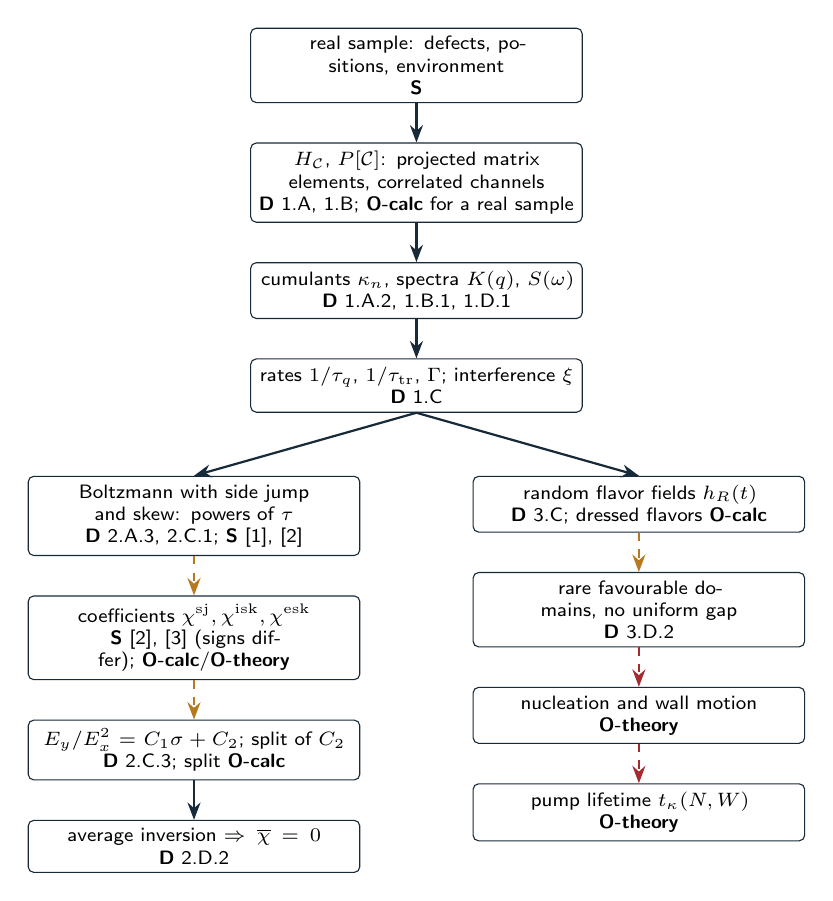
\begin{tikzpicture}[node distance=5mm and 6mm]
\node[obj] (mat) {real sample: defects, positions, environment\\\textbf{S}};
\node[obj,below=of mat] (H) {$H_{\mathcal C}$, $P[\mathcal C]$: projected matrix elements, correlated channels\\\textbf{D} 1.A, 1.B; \textbf{O-calc} for a real sample};
\node[obj,below=of H] (stat) {cumulants $\kappa_n$, spectra $K(q)$, $S(\omega)$\\\textbf{D} 1.A.2, 1.B.1, 1.D.1};
\node[obj,below=of stat] (rates) {rates $1/\tau_q$, $1/\tau_{\rm tr}$, $\Gamma$; interference $\xi$\\\textbf{D} 1.C};
\node[obj,below left=8mm and -14mm of rates] (boltz) {Boltzmann with side jump and skew: powers of $\tau$\\\textbf{D} 2.A.3, 2.C.1; \textbf{S} [1], [2]};
\node[obj,below=of boltz] (coef) {coefficients $\chi^{\rm sj},\chi^{\rm isk},\chi^{\rm esk}$\\\textbf{S} [2], [3] (signs differ); \textbf{O-calc}/\textbf{O-theory}};
\node[obj,below=of coef] (scal) {$E_y/E_x^2=C_1\sigma+C_2$; split of $C_2$\\\textbf{D} 2.C.3; split \textbf{O-calc}};
\node[obj,below=of scal] (avg) {average inversion $\Rightarrow\avg\chi=0$\\\textbf{D} 2.D.2};
\node[obj,below right=8mm and -14mm of rates] (proj) {random flavor fields $h_R(t)$\\\textbf{D} 3.C; dressed flavors \textbf{O-calc}};
\node[obj,below=of proj] (dom) {rare favourable domains, no uniform gap\\\textbf{D} 3.D.2};
\node[obj,below=of dom] (rate) {nucleation and wall motion\\\textbf{O-theory}};
\node[obj,below=of rate] (life) {pump lifetime $t_\kappa(N,W)$\\\textbf{O-theory}};
\draw[okarrow] (mat)--(H); \draw[okarrow] (H)--(stat); \draw[okarrow] (stat)--(rates);
\draw[okarrow] (rates.south)--(boltz.north); \draw[okarrow] (rates.south)--(proj.north);
\draw[calcarrow] (boltz)--(coef); \draw[calcarrow] (coef)--(scal); \draw[okarrow] (scal)--(avg);
\draw[calcarrow] (proj)--(dom); \draw[openarrow] (dom)--(rate); \draw[openarrow] (rate)--(life);
\end{tikzpicture}
\figtext{Black arrows: derived. Amber dashed: open, a calculation is missing (O-calc). Red dashed: open, new theory is needed (O-theory). A third branch (3.A: topology from disorder in a chiral chain, D; interacting long-range average SPT, S [5], [6]; which transport an average symmetry protects, O-theory) is listed in the table below.}
\end{figpanel}

\smallheading{Open links: a calculation or a new theory?}
{\small\begin{longtable}{@{}p{36mm}p{16mm}p{45mm}p{55mm}@{}}\toprule
Open link (questions)&Kind&Closest existing theory&Hypothesis that fails, or the calculation that closes it\\\midrule\endhead
disorder model of a real sample: moments and correlations of its actual defects (1.A, 1.B, 2.D.1)&O-calc&first-principles defect potentials projected on Wannier orbitals; defect statistics from characterization&compute $\delta h$ for each defect type, then $\kappa_n$ and the spectra $K(q)$ for the measured concentrations\\
$\tau^1$ collision coefficients for that disorder (2.C.2, 2.D.3)&O-calc&diagrammatic Kubo theory, non-crossing approximation [3]&evaluate side-jump and intrinsic-skew terms for the real bands and defect T-matrices\\
a semiclassical theory consistent with [3]; coefficients beyond weak disorder (2.C.2(b))&O-theory&Boltzmann theory with side jump [2]; non-crossing diagrammatics [3]&[3] finds contributions without semiclassical counterpart; near the band edge $\hbar/(\eF\tau)$ is not small. Holds for $\eF\tau/\hbar\gg1$ with non-crossing diagrams only\\
collision terms at finite frequency (2.B.3)&O-calc&Kubo or Keldysh theory at finite $\omega$&compute side jump and skew as functions of $\omega\tau$ for the model\\
random fields of the interacting, correlated flavors and of bond disorder over the cycle (3.C)&O-calc&Schrieffer--Wolff dressing; projection as in 3.C.1&compute $h_R(t)$ and the mixings for the many-body flavor states\\
nucleation of reversed domains in rare regions under a slow drive with an alternating field (3.D.2, 3.D.4)&O-theory&Landau--Zener and multiphoton rates; rigorous prethermalization theorems&they need a fast drive or a large uniform gap; here the drive is slow and rare regions have no gap\\
domain-wall motion: pinning versus spreading (3.D.3)&O-theory&random-field Ising wall dynamics (creep) in equilibrium; finite-time tensor-network numerics&creep theory assumes thermal activation; here isolated, periodically driven quantum walls. Holds in the strong-pinning limit\\
Chern number of a two-state manifold in a long disordered ring (3.B.2)&D/O-theory&Niu--Thouless(--Wu) [8]&a gap uniform in $N$, which disorder removes (3.D.2(c)); holds for $N$ below the rare-region spacing\\
transport protected by an average symmetry (2.D.2, 3.A)&O-theory&average-SPT classification of mixed states [14]&the classification concerns ensembles of states, not their driven response; average inversion forbids odd bulk responses\\
\bottomrule\end{longtable}}
\textbf{Shared gap:} in all O-theory links the useful quantity is not an averaged energy or a single broadening but a rate set by rare regions or a constraint set by an ensemble symmetry, and no gap or small parameter is uniform in the system size; a theory of disorder-averaged \emph{dynamics} at this level is missing.

\pagetitle{Appendix B. Source, scope and open conditions for each question}
\smallheading{Problem 1}
\textbf{1.A.1--1.A.2.} Teaching models; the projection $\delta h_{ij}=\langle\varphi_i|v|\varphi_j\rangle$ is the general recipe of tight-binding disorder models. Overlap of the Gaussian orbitals is neglected; with orthogonalized orbitals the numbers change, not the conclusion. Third-order effects: the extrinsic skew term of [1], [2] needs $\kappa_3$ (there $\avg{V_i^3}=V_1^3$).

\textbf{1.B.1--1.B.2.} The tweezer model follows [5], where whole cells are displaced so that the intracell distance is fixed and the long-range dipolar exchange $J_{ij}=C_3(1-3\cos^2\theta_{ij})/(2r_{ij}^3)$ and the van der Waals term both change. The nearest-neighbour, $\theta=90^\circ$ version here is a reduction, not their model.

\textbf{1.C.1--1.C.3.} Weak-disorder Born rates; $\xi=24(4J^2-E^2)a/W^2$ is the perturbative one-dimensional result (it fails near $E=0$, where the exact value is about 10\% larger). The checks of Appendix D confirm both formulas at $W=0.5J$.
\begin{redbox}{O-calc --- what 1.C does not establish}
For a real material, the spectra $K(q)$ and the vertex structure must come from its actual defects; a single $\Gamma$ fitted to a line width is not a disorder model.
\end{redbox}
\textbf{1.D.1--1.D.3.} Classical noise only; quantum baths need ordered correlation functions with $S(\omega)\neq S(-\omega)$ (absorption versus emission) and the bath's own occupation. The puddle estimate assumes local response and uniform fields.

\smallheading{Problem 2}
\textbf{2.A.} Standard [1]. The side-jump coordinate shift is $\delta\bm r_{l'l}=\mathcal A_{l'}-\mathcal A_l-(\nabla_{\bm k}+\nabla_{\bm k'})\arg V_{l'l}$ with the Berry connection $\mathcal A=i\langle u|\nabla u\rangle$; it is gauge invariant only with the phase of the scattering amplitude. [1] groups some $\tau^0$ terms from asymmetric scattering with the side jump; check each paper's naming before comparing.
\begin{greenbox}{[2] --- what the source states}
Formulas for $\chi^{\rm in}$ (the curvature dipole), $\chi^{\rm sj}$, $\chi^{\rm sk,1}$ (intrinsic skew), $\chi^{\rm sk,2}$ (extrinsic skew) of the tilted cone at leading order in the tilt; the ratios in 2.C.2 follow from them. Convention of [2]: $J^{(2)}=\chi\mathcal E\mathcal E$ for the $2\omega$ amplitude and $J=2\chi E^2$ at $\omega=0$; here $\chi$ is the coefficient of $E_x^2$ in $j_y$ (a factor 2), which does not affect ratios. The scaling law of [2] for one static source and its multi-source form with phonons are reproduced in 2.C.3(d).
\end{greenbox}
\begin{redbox}{O-theory --- what 2.C does not establish}
The signs of the collision terms: [3] reverses them relative to [2]. The scaling law survives both; any statement that uses the sign of a collision term (for example ``the total is opposite to the dipole term'') depends on the level of theory.
\end{redbox}
\textbf{2.B.3.} Relaxation-time, intraband, $\hbar\omega\ll2m$. The finite-frequency behaviour of side-jump and skew terms is not given in [2] (low frequency only).

\textbf{2.D.2.} The average-symmetry argument follows the logic of [4]--[6] and [14]; (c) is the ``statistical degeneracy'' of edge states reported in [5]. The selection rule assumes that the clean part is inversion symmetric and that the steady state is a function of the Hamiltonian.

\smallheading{Problem 3}
\textbf{3.A.} The zero-mode recursion and the criterion $\avg{\ln|u|}=\avg{\ln|v|}$ for the disordered chiral chain are exact [15]. It is a toy for ``topology from disorder''; the experiment [5] uses long-range hoppings, van der Waals interactions and average (not exact) inversion.

\textbf{3.B.} B.1 is exact for any configuration. B.2 states the Niu--Thouless theorem [8]; the two-state version (charge $C/q$ for a $q$-fold manifold) is the pumping analogue of the Niu--Thouless--Wu result for degenerate ground states. The displacements $-0.582$ and $-0.418$ are single-particle Wannier-centre data of the clean model at $K/J=-3/2$ (computed in the working folder).

\textbf{3.C.} Fig.\ 3.3 and the table are computed from the clean single-particle chain (24-cell ring, projected-position orbitals of bands 1--2). They are not the dressed, interacting flavors of [7]. The sign alternation of C.3 uses only $H(t+T)=H(t)$ and the flavor exchange, and holds for the interacting flavors as well.
\begin{redbox}{O-calc --- what 3.C does not establish}
The random fields of the correlated flavor states, the effect of bond disorder ($\delta K$, $\delta J$), and the field along the whole cycle for the interacting model.
\end{redbox}
\textbf{3.D.} The domain energy is an effective model consistent with [7], which states $N_c\approx\tilde U/(2\tilde V_{\max})$ and $\ell_{\min}=U/(2\tilde V_{\max})$; the values of $E_{\rm w}$, $\beta_{\max}$, $\sigma_h$, $\gamma$, $\xi$ are illustrative inputs, not results of [7]. The defect model of D.3 is a bookkeeping model.
\begin{redbox}{O-theory --- what 3.D does not establish}
Any lifetime of the disordered pump. D.2 shows that the uniform gap is lost; D.3 shows which time scales with $N$; neither gives a nucleation rate or wall dynamics.
\end{redbox}

\pagetitle{Appendix C. Register of available and missing results}
{\small\begin{tabularx}{\textwidth}{@{}p{42mm}YYp{15mm}@{}}\toprule
Item&Available now&Still missing&Kind\\\midrule
disorder model of a real sample&projection recipe (1.A); position-disorder correlations (1.B)&defect potentials and statistics of the actual sample&O-calc\\
rates and broadening&Born $\tau_q$, $\tau_{\rm tr}$, $\Gamma$, $\xi$ (1.C)&vertex structure and higher cumulants for that sample&O-calc\\
second-order Hall coefficients&powers of $\tau$ (2.C.1); one model in two theories [2], [3]&material-specific coefficients; a consistent semiclassical theory&O-calc / O-theory\\
separation of mechanisms&$C_1$, $C_2$ from scaling (2.C.3)&split of $C_2$; independent $D_x$&O-calc\\
ensemble symmetry&selection rule $\avg\chi=0$; statistical degeneracy (2.D.2)&protected transport of average SPT phases&O-theory\\
flavor fields of the pump&single-particle bias $0.14W$, mixing $0.01W$ (3.C.2)&dressed flavors, bond disorder, full cycle&O-calc\\
domains in the disordered pump&rare favourable blocks, no uniform gap (3.D.2)&nucleation rate, wall motion&O-theory\\
lifetime&scaling of $t_{\rm first}$ and $t_\kappa$ with $N$ (3.D.3)&$t_\kappa(N,W)$ for the real model&O-theory\\
\bottomrule\end{tabularx}}

\pagetitle{Appendix D. Teacher notes}
\smallheading{Provenance and checks}
Every number is recomputed by \texttt{check\_answers.py} (results in \texttt{check\_answers.json}). Independent checks: the golden-rule rate against the exact decay of a plane wave on a 3000-site ring ($0.0234$ vs $0.0241\,J/\hbar$ at $W=0.5J$); the localization length against a transfer-matrix Lyapunov exponent ($283a$ vs $288a$); $\tau_{\rm tr}/\tau_q$ against the exact angular integral ($17.4$ vs $18$); the Berry curvature against a plaquette (Wilson-loop) computation; $D_x$ against a two-dimensional numerical integration ($-8.03$ vs $-8.02\times10^{-4}$ at $v_t=0.02$, $m=0.4$, $\eF=1$); the curvature-dipole coefficient of [2] reproduced from $-(e^3\tau/2\hbar^2)D_x$; Monte Carlo checks of cumulants, bond covariances, mean shifts, puddle averages and $p(4)$; the flavor-orbital weights and the single-period displacements from the clean five-site chain.

\smallheading{Interpretations to confirm}
(i) The sign revision between [2] and [3] is quoted from [3]; 2.C.2(b) uses it only as a hypothetical ``theory II''. (ii) The body of [4] was not available; its content is represented through the original papers [5], [6]. (iii) The identification of the effective domain model of 3.D with the energetics of [7] is ours. (iv) The data of 2.C.3(b) are illustrative.

\smallheading{A priority list for real materials}
For a low-temperature, non-magnetic crystal and a transport or second-order response, a useful first order of checks is: (1) charged impurities and trapped charges, neutral defects, vacancies and alloy disorder (on-site and bond terms, correlated); (2) displaced atoms, strain, thickness or twist-angle variations (essential for narrow bands and small gaps); (3) edges, grain boundaries and surface roughness when the sample is comparable to the mean free path; (4) phonons and other baths when the temperature or the drive supplies energy; (5) slow charge noise and control noise for long observation times (pumps); (6) magnetic impurities and domains whenever the observable depends on a magnetic symmetry. The order is set by the three tests of 1.D.3, not by the size of each term.

\smallheading{Sources}
{\small
[1] N.~Nagaosa, J.~Sinova, S.~Onoda, A.~H.~MacDonald, N.~P.~Ong, Rev.\ Mod.\ Phys.\ 82, 1539 (2010).\
[2] Z.~Z.~Du, C.~M.~Wang, S.~Li, H.-Z.~Lu, X.~C.~Xie, Nat.\ Commun.\ 10, 3047 (2019); arXiv:1812.08377.\
[3] Z.~Z.~Du, C.~M.~Wang, H.-P.~Sun, H.-Z.~Lu, X.~C.~Xie, Nat.\ Commun.\ 12, 5038 (2021); arXiv:2004.09742.\
[4] L.~Hertkorn, Y.~Oreg, Topology from disorder, Nat.\ Phys.\ 22, 1534 (2026).\
[5] Z.~Yue et al., Average topological phase in a disordered Rydberg atom array, Nat.\ Phys.\ (2026); arXiv:2505.06286.\
[6] L.~Su et al., Topological phase transitions and mixed-state order in a Hubbard quantum simulator, Nat.\ Phys.\ (2026); arXiv:2505.17009.\
[7] M.~J\"urgensen, J.~Steiner, G.~Refael, M.~C.~Rechtsman, Multi-band fractional Thouless pumps, arXiv:2504.09338.\
[8] Q.~Niu, D.~J.~Thouless, J.\ Phys.\ A 17, 2453 (1984).\
[9] P.~W.~Anderson, Phys.\ Rev.\ 109, 1492 (1958).\
[10] B.~Kramer, A.~MacKinnon, Rep.\ Prog.\ Phys.\ 56, 1469 (1993).\
[11] S.~Das Sarma, F.~Stern, Phys.\ Rev.\ B 32, 8442 (1985).\
[12] A.~A.~Clerk et al., Rev.\ Mod.\ Phys.\ 82, 1155 (2010).\
[13] J.~Martin et al., Nat.\ Phys.\ 4, 144 (2008).\
[14] R.~Ma, C.~Wang, Phys.\ Rev.\ X 13, 031016 (2023).\
[15] I.~Mondragon-Shem, T.~L.~Hughes, J.~Song, E.~Prodan, Phys.\ Rev.\ Lett.\ 113, 046802 (2014).\
[16] I.~Sodemann, L.~Fu, Phys.\ Rev.\ Lett.\ 115, 216806 (2015).\
[17] Y.~Imry, S.-k.~Ma, Phys.\ Rev.\ Lett.\ 35, 1399 (1975).
}

\clearpage
\pagetitle{Appendix E. Toolbox: the smallest worked examples}
One entry for every tool stated under ``Useful information'' (or in a hint) that is above the reader's level. Each example teaches the tool, not an exam step.

\smallheading{Cumulants (Problem 1, Useful information)}
\textbf{Statement.} $\Cov(x,y)=\avg{xy}-\avg x\avg y$; $\kappa_3=\avg{(x-\avg x)^3}$.\par
\textbf{Smallest example.} $x=0,1,3$ with probabilities $\frac12,\frac14,\frac14$: $\avg x=1$, $\Var x=\frac12\cdot1+0+\frac14\cdot4=1.5$, $\kappa_3=\frac12(-1)+0+\frac14\cdot8=1.5$. Second way: $\avg{x^3}-3\avg x\avg{x^2}+2\avg x^3=7-7.5+2=1.5$.\par
\textbf{Used in} 1.A.2, 1.B.1, 1.B.2, 2.D.1.

\smallheading{Moments of a uniform variable (Problem 1, Useful information)}
\textbf{Statement.} Uniform on $[-W/2,W/2]$: mean 0, variance $W^2/12$, $\kappa_3=0$.\par
\textbf{Smallest example.} $\frac1W\int_{-W/2}^{W/2}x^2\dd x=\frac{W^2}{12}$; the cube is odd, so $\kappa_3=0$. Second way: the uniform variable on $[0,1]$ has variance $\frac13-\frac14=\frac1{12}$.\par
\textbf{Used in} 1.A.2, 1.C.1, 3.C.1.

\smallheading{Golden rule into a quasi-continuum (Problem 1, Useful information)}
\textbf{Statement.} Rate $\frac{2\pi}\hbar\sum_f|V_{fi}|^2\delta(E_f-E_i)$.\par
\textbf{Smallest example.} A level coupled with equal strength $g$ to a ladder of levels with spacing $\delta$: $\sum_f\delta(E_f-E_i)\to1/\delta$, so the rate is $2\pi g^2/(\hbar\delta)$. It describes the decay for times shorter than $2\pi\hbar/\delta$; after that the ladder revives the level.\par
\textbf{Used in} 1.C.1, 1.C.3.

\smallheading{A Fourier sum on a ring (Problem 1, Useful information)}
\textbf{Statement.} $\sum_{j=1}^Le^{i(k-k')j}=L\delta_{kk'}$.\par
\textbf{Smallest example.} $L=3$, $k-k'=2\pi/3$: $e^{2\pi i/3}+e^{4\pi i/3}+1=0$ (the three cube roots of unity); for $k=k'$ the sum is 3.\par
\textbf{Used in} 1.C.1.

\smallheading{Gaussian integrals (Problem 1, Useful information)}
\textbf{Statement.} $\int e^{-\alpha x^2/2}\dd x=\sqrt{2\pi/\alpha}$, $\int x^2e^{-\alpha x^2/2}\dd x=\sqrt{2\pi/\alpha}/\alpha$.\par
\textbf{Smallest example.} $\alpha=1$: the ratio of the two integrals is $1$, the variance of a standard Gaussian. Second way: differentiate the first integral with respect to $\alpha$.\par
\textbf{Used in} 1.C.2.

\smallheading{Noise spectrum and transition rate (Problem 1, Useful information)}
\textbf{Statement.} $S(\omega)=\int e^{i\omega t}\avg{\eta(t)\eta(0)}\dd t$; rate $|A_{10}|^2S(\omega_0)/\hbar^2$.\par
\textbf{Smallest example.} For $\avg{\eta(t)\eta(0)}=\sigma^2e^{-|t|/\tau_{\rm c}}$: $S=2\sigma^2\,\mathrm{Re}\int_0^\infty e^{(i\omega-1/\tau_{\rm c})t}\dd t=2\sigma^2\,\mathrm{Re}\frac1{1/\tau_{\rm c}-i\omega}=\frac{2\sigma^2\tau_{\rm c}}{1+\omega^2\tau_{\rm c}^2}$. Check: $\int S\,\dd\omega/2\pi=\sigma^2$, the variance.\par
\textbf{Used in} 1.D.1.

\smallheading{Averages of a function of a random variable (Problem 1, Useful information)}
\textbf{Statement.} $\avg{F(x)}\approx F(0)+\frac12F''(0)\avg{x^2}$, $\Var F\approx F'(0)^2\avg{x^2}$.\par
\textbf{Smallest example.} $F=x+x^2$, Gaussian $x$ of variance $\sigma^2$: $\avg F=\sigma^2$ exactly, as the formula gives; $\Var F=\sigma^2+2\sigma^4$, whose leading term $\sigma^2$ is the formula.\par
\textbf{Used in} 1.B.2, 1.D.2.

\smallheading{Berry curvature of a two-band Hamiltonian (Problem 2, Useful information)}
\textbf{Statement.} $\Omega_\pm=\mp\bm d\cdot(\partial_{k_x}\bm d\times\partial_{k_y}\bm d)/(2|\bm d|^3)$.\par
\textbf{Smallest example.} $\bm d=(k_x,k_y,1)$ at $\bm k=0$: $\Omega_\pm=\mp\frac12$. Second way: $\int\Omega_-\,\dd^2k/2\pi=\frac12$, half of the solid angle $4\pi$ divided by $4\pi$ --- the vector $\hat{\bm d}$ covers one hemisphere.\par
\textbf{Used in} 2.A.1.

\smallheading{Delta function of a function; polar integrals (Problem 2, Useful information)}
\textbf{Statement.} $\delta(G(k))=\delta(k-k_0)/|\dd G/\dd k|_{k_0}$; $\int\dd^2k\,F(k)=2\pi\int Fk\,\dd k$; $\int\cos^2\phi\,\dd\phi=\pi$.\par
\textbf{Smallest example.} $\int_0^\infty\delta(k^2-1)\,\dd k=\frac12$. $\int\dd^2k\,k_x^2e^{-k^2}=\pi\int_0^\infty k^3e^{-k^2}\dd k=\frac\pi2$; second way: $\int k_x^2e^{-k_x^2}\dd k_x\int e^{-k_y^2}\dd k_y=\frac{\sqrt\pi}2\sqrt\pi$.\par
\textbf{Used in} 2.A.1, 2.B.2.

\smallheading{Integration by parts in $\bm k$ (Problem 2, Useful information)}
\textbf{Statement.} $\int f\partial_{k_x}g=-\int g\partial_{k_x}f$ if $fg\to0$.\par
\textbf{Smallest example.} One dimension, $f=e^{-k^2}$, $g=k$: $\int f\,\dd k=\sqrt\pi$ and $-\int k(-2k)e^{-k^2}\dd k=\sqrt\pi$.\par
\textbf{Used in} 2.B.1, 2.B.2.

\smallheading{Products of oscillating quantities (Problem 2, Useful information)}
\textbf{Statement.} $\mathrm{Re}(\alpha e^{i\omega t})\mathrm{Re}(\beta e^{i\omega t})=\frac12\mathrm{Re}(\alpha\beta e^{2i\omega t})+\frac12\mathrm{Re}(\alpha\beta^*)$.\par
\textbf{Smallest example.} $\alpha=\beta=1$: $\cos^2\omega t=\frac12+\frac12\cos2\omega t$. With $\beta=i$: $-\cos\omega t\sin\omega t=-\frac12\sin2\omega t$ and the constant part vanishes.\par
\textbf{Used in} 2.B.3.

\smallheading{Heisenberg equation for fermion densities (Problem 3, Useful information)}
\textbf{Statement.} $\dot O=i[H,O]$; $[c_a^\dagger c_b,n_j]=c_a^\dagger c_b(\delta_{bj}-\delta_{aj})$.\par
\textbf{Smallest example.} Two sites, $H=-J(c_2^\dagger c_1+c_1^\dagger c_2)$: $\dot n_1=-iJ(c_2^\dagger c_1-c_1^\dagger c_2)$. For the bonding state $(\ket1+\ket2)/\sqrt2$ the expectation value is zero (a stationary state); for $(\ket1+i\ket2)/\sqrt2$ it is $-J$, a particle flowing from 1 to 2.\par
\textbf{Used in} 3.B.1.

\smallheading{Law of large numbers for products (Problem 3, Useful information)}
\textbf{Statement.} $\frac1n\sum\ln|x_i|\to\avg{\ln|x|}$; $\int\ln x\,\dd x=x\ln x-x$.\par
\textbf{Smallest example.} $x=\frac12$ or $2$ with equal probability: $\avg x=1.25>1$, but $\avg{\ln x}=0$, so a long product neither grows nor decays exponentially --- its typical size is set by the logarithmic mean. And $\int_0^1\ln x\,\dd x=-1$.\par
\textbf{Used in} 3.A.1, 3.A.2.

\smallheading{Pauli decomposition (Problem 3, Useful information)}
\textbf{Statement.} $M=h_0\id+\bm h\cdot\bm s$ with $h_z=(M_{11}-M_{22})/2$, $h_x-ih_y=M_{12}$.\par
\textbf{Smallest example.} $M=\begin{pmatrix}3&1-i\\1+i&1\end{pmatrix}$: $h_0=2$, $h_z=1$, $h_x=h_y=1$. Second way: the eigenvalues $h_0\pm|\bm h|=2\pm\sqrt3$ equal those of $M$.\par
\textbf{Used in} 3.C.1, 3.C.2.

\smallheading{Gaussian sums and $\Phi$ (Problem 3, Useful information)}
\textbf{Statement.} A sum of $\ell$ independent Gaussians of variance $\sigma^2$ has variance $\ell\sigma^2$; $\Phi(-1)=0.159$.\par
\textbf{Smallest example.} Four standard Gaussians: the sum has rms 2, so $P(\text{sum}>2)=\Phi(-1)=0.159$.\par
\textbf{Used in} 3.D.2.

\smallheading{Independent rare events (Problem 3, Useful information)}
\textbf{Statement.} Probability of no event in time $t$: $e^{-\Lambda t}$.\par
\textbf{Smallest example.} Two independent sources, each at rate $\Lambda/2$: no event in either, $e^{-\Lambda t/2}e^{-\Lambda t/2}=e^{-\Lambda t}$ --- rates of independent sources add.\par
\textbf{Used in} 3.D.3.

\vfill
\begin{center}\textbf{End of solution booklet}\end{center}
\end{document}
